% advsync/advsync.tex
% mainfile: ../perfbook.tex
% SPDX-License-Identifier: CC-BY-SA-3.0

\QuickQuizChapter{sec:advsync:Advanced Synchronization}{Advanced Synchronization}{qqzadvsync}
%
\Epigraph{If a little knowledge is a dangerous thing, just think what
	  you could do with a lot of knowledge!}{\emph{Unknown}}

This chapter covers synchronization techniques used for lockless
algorithms and parallel real-time systems.

Although lockless algorithms can be quite helpful when faced with
extreme requirements, they are no panacea.
For example, as noted at the end of \cref{chp:Counting},
you should thoroughly apply partitioning, batching, and
well-tested packaged weak APIs
(see \cref{chp:Data Ownership,chp:Deferred Processing})
before even thinking about lockless algorithms.

But after doing all that, you still might find yourself needing the
advanced techniques described in this chapter.
To that end,
\cref{sec:advsync:Avoiding Locks}
summarizes techniques used thus far for avoiding locks and
\cref{sec:advsync:Non-Blocking Synchronization}
gives a brief overview of non-blocking synchronization.
Memory ordering is also quite important, but it warrants its own
\lcnamecref{chp:Advanced Synchronization: Memory Ordering}, namely
\cref{chp:Advanced Synchronization: Memory Ordering}.

The second form of advanced synchronization provides the stronger
\IXpl{forward-progress guarantee} needed for parallel real-time computing,
which is the topic of
\cref{sec:advsync:Parallel Real-Time Computing}.

\section{Avoiding Locks}
\label{sec:advsync:Avoiding Locks}
%
\epigraph{We are confronted with insurmountable opportunities.}
	 {\emph{Walt Kelly}}

Although locking is the workhorse of parallelism in production, in
many situations performance, scalability, and real-time response can
all be greatly improved through use of lockless techniques.
A particularly impressive example of such a lockless technique is
the statistical counters described in
\cref{sec:count:Statistical Counters},
which avoids not only locks, but also atomic operations, memory barriers,
and even cache misses for counter increments.
Other examples we have covered include:

\begin{enumerate}
\item	The fastpaths through a number of other counting algorithms
	in \cref{chp:Counting}.
\item	The fastpath through resource allocator caches in
	\cref{sec:SMPdesign:Resource Allocator Caches}.
\item	The maze solver in \cref{sec:SMPdesign:Beyond Partitioning}.
\item	The data-ownership techniques in \cref{chp:Data Ownership}.
\item	The reference-counting, hazard-pointer, and RCU techniques
	in \cref{chp:Deferred Processing}.
\item	The lookup code paths in \cref{chp:Data Structures}.
\item	Many of the techniques in \cref{chp:Putting It All Together}.
\end{enumerate}

In short, lockless techniques are quite useful and are heavily used.
However, it is best if lockless techniques are hidden behind a
well-defined API, such as the \co{inc_count()}, \co{memblock_alloc()},
\co{rcu_read_lock()}, and so on.
The reason for this is that undisciplined use of lockless techniques
is a good way to create difficult bugs.
If you believe that finding and fixing such bugs is easier than avoiding
them, please re-read
\cref{chp:Validation,chp:Formal Verification}.

\section{Non-Blocking Synchronization}
\label{sec:advsync:Non-Blocking Synchronization}
%
\epigraph{Never worry about theory as long as the machinery does what
	  it's supposed to do.}
	 {\emph{Robert A. Heinlein}}

The term \IXacrfst{nbs}~\cite{MauriceHerlihy90a}
describes seven classes of linearizable algorithms with differing
\emph{\IXpl{forward-progress guarantee}}~\cite{DanAlitarh2013PracticalProgress},
which are as follows:

\begin{enumerate}
\item	\emph{\IXalth{Bounded wait-free}{bounded}{wait free} synchronization}:
	Every thread will make progress within
	a specific finite period of time~\cite{Herlihy91}.
	This level is widely considered to be unachievable, which might be why
	Alitarh et al.\ omitted it~\cite{DanAlitarh2013PracticalProgress}.
\item	\emph{\IXalt{Wait-free}{wait free} synchronization}:
	Every thread will make progress
	in finite time~\cite{Herlihy93}.
\item	\emph{\IXalt{Lock-free}{lock free} synchronization}:
	At least one thread will
	make progress in finite time~\cite{Herlihy93}.
\item	\emph{\IXalt{Obstruction-free}{obstruction free} synchronization}:
	Every thread will make progress in finite time in the absence of
	contention~\cite{HerlihyLM03}.
\item	\emph{\IXalt{Clash-free}{clash free} synchronization}:
	At least one thread will make progress in finite time in the absence of
	contention~\cite{DanAlitarh2013PracticalProgress}.
\item	\emph{\IXalt{Starvation-free}{starvation free} synchronization}:
	Every thread will make progress in finite time in the absence of
	failures~\cite{DanAlitarh2013PracticalProgress}.
\item	\emph{\IXalt{Deadlock-free}{deadlock free} synchronization}:
	At least one thread will make progress in finite time in the absence of
	failures~\cite{DanAlitarh2013PracticalProgress}.
\end{enumerate}

NBS classes~1, 2, and~3 were first formulated in the early 1990s,
class~4 was first formulated in the early 2000s,
and class~5 was first formulated in 2013.
The final two classes have seen informal use for a great many decades,
but were reformulated in 2013.

In theory, any parallel algorithm can be cast into wait-free form,
but there are a relatively small subset of NBS algorithms that are
in common use.
A few of these are listed in the following section.

\subsection{Simple NBS}
\label{sec:advsync:Simple NBS}

Perhaps the simplest NBS algorithm is atomic update of an integer
counter using fetch-and-add (\co{atomic_add_return()}) primitives.

\subsubsection{NBS Sets}
\label{sec:advsync:NBS Sets}

Another simple NBS algorithm implements a set of integers in an array.
Here the array index indicates a value that might be a member of the set
and the array element indicates whether or not that value actually is
a set member.
The linearizability criterion for NBS algorithms requires that reads from
and updates to the array either use atomic instructions or be accompanied
by memory barriers, but in the not-uncommon case where linearizability
is not important, simple volatile loads and stores suffice, for example,
using \co{READ_ONCE()} and \co{WRITE_ONCE()}.

An NBS set may also be implemented using a bitmap, where each value that
might be a member of the set corresponds to one bit.
Reads and updates must normally be carried out via atomic bit-manipulation
instructions, although compare-and-swap (\co{cmpxchg()} or CAS)
instructions can also be used.

\subsubsection{NBS Counters}
\label{sec:advsync:NBS Counters}

The statistical counters algorithm discussed in
\cref{sec:count:Statistical Counters}
can be considered to be bounded-wait-free, but only by using a cute
definitional trick in which the sum is considered to be approximate
rather than exact.\footnote{
	Citation needed.
	I heard of this trick verbally from Mark Moir.}
Given sufficiently wide error bounds that are a function of the length
of time that the \co{read_count()} function takes to sum the counters,
it is not possible to prove that any non-linearizable behavior occurred.
This definitely (if a bit artificially) classifies the statistical-counters
algorithm as bounded wait-free.
This algorithm is probably the most heavily used NBS algorithm in the
Linux kernel.

\subsubsection{Half-NBS Queue}
\label{sec:advsync:Half-NBS Queue}

\begin{fcvref}[ln:count:NBS Enqueue Algorithm]
Another common NBS algorithm is the atomic queue where elements are
enqueued using an atomic exchange instruction~\cite{MagedMichael1993JPDC},
followed by a store into the \co{->next} pointer of the new element's
predecessor, as shown in \cref{lst:count:NBS Enqueue Algorithm},
which shows the userspace-RCU library
implementation~\cite{MathieuDesnoyers2009URCU}.
\Clnref{tail} updates the tail pointer to reference the new element while
returning a reference to its predecessor, which is stored in
local variable \co{old_tail}.
\Clnref{pred} then updates the predecessor's \co{->next} pointer to
reference the newly added element, and finally \clnref{ret}
returns an indication as to whether or not the queue was initially
empty.

\begin{listing}
\begin{fcvlabel}[ln:count:NBS Enqueue Algorithm]
\begin{VerbatimL}[commandchars=\\\[\]]
static inline bool
___cds_wfcq_append(struct cds_wfcq_head *head,
                   struct cds_wfcq_tail *tail,
                   struct cds_wfcq_node *new_head,
                   struct cds_wfcq_node *new_tail)
{
	struct cds_wfcq_node *old_tail;

	old_tail = uatomic_xchg(&tail->p, new_tail);	\lnlbl[tail]
	CMM_STORE_SHARED(old_tail->next, new_head);     \lnlbl[pred]
	return old_tail != &head->node;			\lnlbl[ret]
}

static inline bool
_cds_wfcq_enqueue(struct cds_wfcq_head *head,
                  struct cds_wfcq_tail *tail,
                  struct cds_wfcq_node *new_tail)
{
	return ___cds_wfcq_append(head, tail,
	                          new_tail, new_tail);
}
\end{VerbatimL}
\end{fcvlabel}
\caption{NBS Enqueue Algorithm}
\label{lst:count:NBS Enqueue Algorithm}
\end{listing}

Although mutual exclusion is required to dequeue a single element
(so that dequeue is blocking), it is possible to carry out a non-blocking
removal of the entire contents of the queue.
What is not possible is to dequeue any given element in a non-blocking
manner: The enqueuer might have failed between \clnref{tail,pred} of the
listing, so that the element in question is only partially enqueued.
This results in a half-NBS algorithm where enqueues are NBS but
dequeues are blocking.
This algorithm is nevertheless heavily used in practice, in part because
most production software is not required to tolerate arbitrary fail-stop
errors.
\end{fcvref}

\subsubsection{NBS Stack}
\label{sec:advsync:NBS Stack}

\begin{fcvref}[ln:advsync:lifo_push:whole]
\Cref{lst:advsync:NBS Stack Algorithm}
shows the LIFO push algorithm, which boasts lock-free push and
bounded wait-free pop (\path{lifo-push.c}), forming an NBS stack.
The origins of this algorithm are unknown, but it was referred to in
a patent granted in 1975~\cite{PaulJBrown1975LIFOpush}.
This patent was filed in 1973, a few months before your editor
saw his first computer, which had but one CPU\@.

\begin{listing}
\input{CodeSamples/advsync/lifo_push@whole.fcv}
\caption{NBS Stack Algorithm}
\label{lst:advsync:NBS Stack Algorithm}
\end{listing}

\Clnrefrange{struct:b}{struct:e} show the \co{node_t} structure,
which contains an arbitrary value and a pointer to the next structure
on the stack and
\clnref{top} shows the top-of-stack pointer.

The \co{list_push()} function spans \clnrefrange{push:b}{push:e}.
\Clnref{push:alloc} allocates a new node and
\clnref{push:initialize} initializes it.
\Clnref{push:next} initializes the newly allocated node's \co{->next}
pointer, and \clnref{push:cmpxchg} attempts to push it on the stack.
If \clnref{push:check} detects \co{cmpxchg()} failure, another pass
through the loop retries.
Otherwise, the new node has been successfully pushed, and this function
returns to its caller.
Note that \clnref{push:check} resolves races in which two concurrent
instances of \co{list_push()} attempt to push onto the stack.
The \co{cmpxchg()} will succeed for one and fail for the other,
causing the other to retry, thereby selecting an arbitrary order for
the two node on the stack.

The \co{list_pop_all()} function spans \clnrefrange{popall:b}{popall:e}.
The \co{xchg()} statement on \clnref{popall:xchg} atomically removes
all nodes on the stack, placing the head of the resulting list in local
variable \co{p} and setting \co{top} to \co{NULL}.
This atomic operation serializes concurrent calls to \co{list_pop_all()}:
One of them will get the list, and the other a \co{NULL} pointer, at
least assuming that there were no concurrent calls to \co{list_push()}.

An instance of \co{list_pop_all()} that obtains a non-empty list in
\co{p} processes this list in the loop spanning
\clnrefrange{popall:loop:b}{popall:loop:e}.
\Clnref{popall:next} prefetches the \co{->next} pointer,
\clnref{popall:foo} invokes the function referenced by \co{foo()} on the
current node,
\clnref{popall:free} frees the current node, and
\clnref{popall:pnext} sets up \co{p} for the next pass through the loop.

But suppose that a pair of \co{list_push()} instances run concurrently
with a \co{list_pop_all()} with a list initially containing a single
\Node{A}.
Here is one way that this scenario might play out:

\begin{enumerate}
\item	The first \co{list_push()} instance pushes a new \Node{B},
	executing through \clnref{push:next}, having just stored
	a pointer to \Node{A} into \Node{B}'s \co{->next} pointer.
\item	The \co{list_pop_all()} instance runs to completion,
	setting \co{top} to \co{NULL} and freeing \Node{A}.
\item	The second \co{list_push()} instance runs to completion,
	pushing a new \Node{C}, but happens to allocate the memory
	that used to belong to \Node{A}.
\item	The first \co{list_push()} instance executes the \co{cmpxchg()}
	on \clnref{push:cmpxchg}.
	Because new \Node{C} has the same address as the newly freed \Node{A},
	this \co{cmpxchg()} succeeds and this \co{list_push()} instance
	runs to completion.
\end{enumerate}

Note that both pushes and the popall all ran successfully despite the
reuse of \Node{A}'s memory.
This is an unusual property: Most data structures require protection
against what is often called the ABA problem.

But this property holds only for algorithm written in assembly
language.
The sad fact is that most languages (including C and C++) do not support
pointers to lifetime-ended objects, such as the pointer to the old \Node{A}
contained in \Node{B}'s \co{->next} pointer.
In fact, compilers are within their rights to assume that if two pointers
(call them \co{p} and \co{q}) were returned from two different calls to
\co{malloc()}, then those pointers must not be equal.
Real compilers really will generate the constant \co{false} in
response to a \co{p==q} comparison.
A pointer to an object that has been freed, but whose memory has been
reallocated for a compatibly typed object is termed a \emph{zombie pointer}.

Many concurrent applications avoid this problem by carefully hiding the
memory allocator from the compiler, thus preventing the compiler from
making inappropriate assumptions.
This obfuscatory approach currently works in practice, but might well
one day fall victim to increasingly aggressive optimizers.
There is work underway in both the C and C++ standards committees
to address this
problem~\cite{PaulEMcKenney2019PointerLifetimeEndZap,PaulEMcKenney2020PointerLifetimeEndZapCpp}.
In the meantime, please exercise great care when coding ABA-tolerant
algorithms.
\end{fcvref}

\QuickQuiz{
	So why not ditch antique languages like C and C++ for something
	more modern?
}\QuickQuizAnswer{
	That won't help unless the more-modern languages proponents
	are energetic enough to write their own compiler backends.
	The usual practice of re-using existing backends also reuses
	charming properties such as refusal to support pointers to
	lifetime-ended objects.
}\QuickQuizEnd

\subsection{Applicability of NBS Benefits}
\label{sec:advsync:Applicability of NBS Benefits}

The most heavily cited NBS benefits stem from its forward-progress
guarantees, its tolerance of fail-stop bugs, and from its linearizability.
Each of these is discussed in one of the following sections.

\subsubsection{NBS Forward Progress Guarantees}
\label{sec:advsync:NBS Forward Progress Guarantees}

NBS's forward-progress guarantees have caused many to suggest its use in
real-time systems, and NBS algorithms are in fact used in a great many
such systems.
However, it is important to note that forward-progress guarantees are
largely orthogonal to those that form the basis of real-time programming:

\begin{enumerate}
\item	Real-time forward-progress guarantees usually have some
	definite time associated with them, for example,
	``scheduling latency must be less than 100 microseconds.''
	In contrast, the most popular forms of NBS only guarantees
	that progress will be made in finite time, with no definite
	bound.
\item	Real-time forward-progress guarantees are often
	probabilistic, as in the soft-real-time guarantee that
	``at least 99.9\,\% of the time, scheduling latency must
	be less than 100 microseconds.''
	In contrast, many of NBS's forward-progress guarantees are
	unconditional.
\item	Real-time forward-progress guarantees are often conditioned on
	environmental constraints, for example, only being honored:
	(1)~For the highest-priority tasks,
	(2)~When each CPU spends at least a certain fraction of its time idle,
	and (3)~When I/O rates are below some specified maximum.
	In contrast, NBS's forward-progress
	guarantees are often unconditional, although recent NBS work
	accommodates conditional
	guarantees~\cite{DanAlitarh2013PracticalProgress}.
\item	An important component of a real-time program's environment
	is the scheduler.
	NBS algorithms assume a worst-case \emph{demonic scheduler}.
	In contrast, real-time systems assume that the scheduler is
	doing its level best to satisfy any scheduling constraints
	it knows about, and, in the absence of such constraints,
	its level best to honor process priorities and to provide
	fair scheduling to processes of the same priority.
	This assumption of a non-demonic scheduler allows real-time
	programs to use simpler algorithms than those required for
	NBS~\cite{DanAlitarh2013PracticalProgress,BjoernBrandenburgPhD}.
\item	Real-time forward-progress guarantees usually apply only
	in the absence of software bugs.
	In contrast, many classes of NBS guarantees apply even in the
	face of fail-stop bugs.
\item	NBS forward-progress guarantee classes imply linearizability.
	In contrast, real-time forward progress guarantees are often
	independent of ordering constraints such as linearizability.
\end{enumerate}

To reiterate, despite these differences, a number of NBS algorithms are
extremely useful in real-time programs.

\subsubsection{NBS Fail-Stop Tolerance}
\label{sec:advsync:NBS Fail-Stop Tolerance}

Of the classes of NBS algorithms, wait-free synchronization (bounded or
otherwise), lock-free synchronization, obstruction-free synchronization,
and clash-free synchronization guarantee forward progress even in the
presence of fail-stop bugs.
An example fail-stop bug might cause some thread to be preempted indefinitely.
As we will see, this fail-stop-tolerant property can be useful, but the
fact is that composing a set of fail-stop-tolerant mechanisms does not
necessarily result in a fail-stop-tolerant system.
To see this, consider a system made up of a series of wait-free queues,
where an element is removed from one queue in the series, processed,
and then added to the next queue.

If a thread is preempted in the midst of a queuing operation, in theory
all is well because the wait-free nature of the queue will guarantee
forward progress.
But in practice, the element being processed is lost because the
fail-stop-tolerant nature of the wait-free queues does not extend to
the code using those queues.

Nevertheless, there are a few applications where NBS's rather limited
fail-stop-tolerance is useful.
For example, in some network-based or web applications, a fail-stop
event will eventually result in a retransmission, which will restart
any work that was lost due to the fail-stop event.
Systems running such applications can therefore be heavily loaded, even
to the point where the scheduler can no longer provide any reasonable
fairness guarantee.
In constrast, if a thread fail-stops while holding a lock, the application
might need to be restarted.
Nevertheless, NBS is not a panacea even within this restricted area,
due to the possibility of spurious retransmissions due to pure scheduling
delays.
In some cases, it may be more efficient to reduce the load to avoid
queueing delays, which will also improve the scheduler's ability to
provide fair access, reducing or even eliminating the fail-stop events,
thus reducing the number of retry operations, in turn further reducing
the load.

\subsubsection{NBS Linearizability}
\label{sec:advsync:NBS Linearizability}

It is important to note that linearizability can be quite useful,
especially when analyzing concurrent code made up of strict locking
and fully ordered atomic operations.\footnote{
	For example, the Linux kernel's value-returning atomic operations.}
Furthermore, this handling of fully ordered atomic operations
automatically covers simple NBS algorithms.

However, the linearization points of a complex NBS algorithms are often
buried deep within that algorithm, and thus not visible to users of
a library function implementing a part of such an algorithm.
Therefore, any claims that users benefit from the linearizability properties
of complex NBS algorithms should be regarded with deep
suspicion~\cite{AndreasHaas2012FIFOisnt}.

It is sometimes asserted that linearizability is necessary for developers
to produce proofs of correctness for their concurrent code.
However, such proofs are the exception rather than the rule, and modern
developers who do produce proofs often use modern proof techniques that
do not depend on linearizability.
Furthermore, developers frequently use modern proof techniques that do
not require a full specification, given that developers often learn
their specification after the fact, one bug at a time.
A few such proof techniques were discussed in
\cref{chp:Formal Verification}.\footnote{
	A memorable verbal discussion with an advocate of linearizability
	resulted in question:
	``So the reason linearizability is important is to rescue 1980s
	proof techniques?''
	The advocate immediately replied in the affirmative, then spent
	some time disparaging a particular modern proof technique.
	Oddly enough, that technique was one of those successfully
	applied to Linux-kernel RCU\@.}

It is often asserted that linearizability maps well to sequential
specifications, which are said to be more natural than are concurrent
specifications~\cite{SergioRajsbaum2020HistoryLinearizability}.
But this assertion fails to account for our highly concurrent objective
universe.
This universe can only be expected to select for ability to cope with
concurrency, especially for those participating in team sports or
overseeing small children.
In addition, given that the teaching of sequential
computing is still believed to be somewhat of a black
art~\cite{ElizabethPatitsas2020GradesNotBimodal}, it is reasonable
to expect that teaching of concurrent computing is in a similar state
of disarray.
Therefore, focusing on only one proof technique is unlikely to be a
good way forward.

Again, please understand that linearizability is quite useful in many
situations.
Then again, so is that venerable tool, the hammer.
But there comes a point in the field of computing where one should put
down the hammer and pick up a keyboard.
Similarly, it appears that there are times when linearizability is not
the best tool for the job.

To their credit, there are some linearizability advocates who are aware
of some of its shortcomings~\cite{SergioRajsbaum2020HistoryLinearizability}.
There are also proposals to extend linearizability, for example,
interval-linearizability, which is intended to handle the common case
of operations that require non-zero time to
complete~\cite{10.1145/3266457}.
It remains to be seen whether these proposals will result in theories
able to handle modern concurrent software artifacts, especially given
that several of the proof techniques discussed in \cref{chp:Formal
Verification} already handle many modern concurrent software artifacts.

\subsection{NBS Discussion}
\label{sec:advsync:NBS Discussion}

It is possible to create fully non-blocking queues~\cite{MichaelScott96},
however, such queues are much more complex than the half-NBS algorithm
outlined above.
The lesson here is to carefully consider your actual requirements.
Relaxing irrelevant requirements can often result in great
improvements in simplicity, performance, and scalability.

Recent research points to another important way to relax requirements.
It turns out that systems providing fair scheduling can enjoy most
of the benefits of wait-free synchronization even when running
algorithms that provide only non-blocking
synchronization, both in theory~\cite{DanAlitarh2013PracticalProgress}
and in practice~\cite{SamyAlBahra2013NBS}.
Because most schedulers used in production do in fact provide fairness,
the more-complex algorithms providing wait-free synchronization usually
provide no practical advantages over simpler and faster non-wait-free
algorithms.

Interestingly enough, fair scheduling is but one beneficial
constraint that is often respected in practice.
Other sets of constraints can permit blocking algorithms to
achieve deterministic real-time response.
For example, given:
(1)~Fair locks granted in FIFO order within a given priority level,
(2)~Priority inversion avoidance (for example, priority
inheritance~\cite{Takada:1995:RSN:527074.828566,Cai-DongWang1996PrioInherLock}
or priority ceiling),
(3)~A bounded number of threads,
(4)~Bounded critical section durations,
(5)~Bounded load,
and
(6)~Absence of fail-stop bugs,
lock-based applications can provide deterministic
response times~\cite{BjoernBrandenburgPhD,DipankarSarma2004OLSscalability}.
This approach of course blurs the distinction between blocking and wait-free
synchronization, which is all to the good.
Hopefully theoretical frameworks will continue to improve their ability
to describe software actually used in practice.

Those who feel that theory should lead the way are referred to the
inimitable Peter Denning, who said of operating systems:
``Theory follows practice''~\cite{Denning:2015:POF:2830903.2830904},
or to the eminent Tony Hoare, who said of the whole of engineering:
``In all branches of engineering science, the engineering starts before
the science; indeed, without the early products of engineering, there
would be nothing for the scientist to
study!''~\cite{RichardMorris2007TonyHoareInterview}.
However, once an appropriate body of theory becomes available,\footnote{
	Note well that the first \emph{appropriate} body of theory is often one
	thing and the first \emph{proposed} body of theory quite another.}
it is wise to make use of it.

% advsync/rt.tex
% mainfile: ../perfbook.tex
% SPDX-License-Identifier: CC-BY-SA-3.0

\section{Parallel Real-Time Computing}
\label{sec:advsync:Parallel Real-Time Computing}
%
\epigraph{One always has time enough if one applies it well.}
	 {Johann Wolfgang von G\"othe}
% \epigraph{The difference between you and me is that I was right in time.}
% 	 {Konrad Adenauer}
% No support for this quote found.

An important emerging area in computing is that of parallel real-time
computing.
\Cref{sec:advsync:What is Real-Time Computing?}
looks at a number of definitions of ``real-time computing'', moving
beyond the usual sound bites to more meaningful criteria.
\Cref{sec:advsync:Who Needs Real-Time?}
surveys the sorts of applications that need real-time response.
\Cref{sec:advsync:Who Needs Parallel Real-Time?}
notes that parallel real-time computing is upon us, and discusses
when and why parallel real-time computing can be useful.
\Cref{sec:advsync:Implementing Parallel Real-Time Systems}
gives a brief overview of how parallel real-time systems may be implemented,
with
\cref{sec:advsync:Implementing Parallel Real-Time Operating Systems,%
sec:advsync:Implementing Parallel Real-Time Applications}
focusing on operating systems and applications, respectively.
Finally,
\cref{sec:advsync:Real Time vs. Real Fast: How to Choose?}
outlines how to decide whether or not your application needs real-time
facilities.

\subsection{What is Real-Time Computing?}
\label{sec:advsync:What is Real-Time Computing?}

One traditional way of classifying real-time computing is into the
categories of \emph{hard real time} and \emph{soft real time}, where
the macho hard real-time applications never miss their deadlines, but
the wimpy soft real-time applications miss their deadlines quite often.

\subsubsection{Soft Real Time}
\label{sec:Soft Real Time}

It should be easy to see problems with this definition of soft real time.
For one thing, by this definition, \emph{any} piece of software could be
said to be a soft real-time application:
``My application computes million-point Fourier transforms in half a
picosecond.''
``No way!!!
The clock cycle on this system is more than \emph{three hundred} picoseconds!''
``Ah, but it is a \emph{soft} real-time application!''
If the term ``soft real time'' is to be of any use whatsoever, some limits
are clearly required.

We might therefore say that a given soft real-time application must meet
its response-time requirements at least some fraction of the time, for
example, we might say that it must execute in less than 20 microseconds
99.9\,\% of the time.

This of course raises the question of what is to be done when the application
fails to meet its response-time requirements.
The answer varies with the application, but one possibility
is that the system being controlled has sufficient stability and inertia
to render harmless the occasional late control action.
Another possibility is that the application has two ways of computing
the result, a fast and deterministic but inaccurate method on the
one hand and
a very accurate method with unpredictable compute time on the other.
One reasonable approach would be to start
both methods in parallel, and if the accurate method fails to finish
in time, kill it and use the answer from the fast but inaccurate method.
One candidate for the fast but inaccurate method is to take
no control action during the current time period, and another candidate is
to take the same control action as was taken during the preceding time
period.

In short, it does not make sense to talk about soft real time without
some measure of exactly how soft it is.

\subsubsection{Hard Real Time}
\label{sec:Hard Real Time}

In contrast, the definition of hard real time is quite definite.
After all, a given system either always meets its deadlines or it
doesn't.

\begin{figure}
\centering
\resizebox{3in}{!}{\includegraphics{cartoons/realtime-smash}}
\caption{Real-Time Response, Meet Hammer}
\ContributedBy{Figure}{fig:advsync:Hard Real-Time Response; Meet Hammer}{Melissa Broussard}
\end{figure}

Unfortunately, a strict application of this definition would mean that
there can never be any hard real-time systems.
The reason for this is fancifully depicted in
\cref{fig:advsync:Hard Real-Time Response; Meet Hammer}.
And although you can always construct a more robust system, perhaps with
redundancy, your adversary can always get a bigger hammer.
But don't take \emph{my} word for it:
Ask the dinosaurs.

\begin{figure}
\centering
\resizebox{3in}{!}{\includegraphics{cartoons/realtime-lifesupport-nobomb}}
\caption{Real-Time Response:
			     Hardware Matters}
\ContributedBy{Figure}{fig:advsync:Real-Time Response: Hardware Matters}{Melissa Broussard}
\end{figure}

Then again, perhaps it is unfair to blame the software for what is clearly
not just a hardware problem, but a bona fide big-iron hardware problem
at that.\footnote{
	Or, given modern hammers, a big-steel problem.}
This suggests that we define hard real-time software as software that
will always meet its deadlines, but only in the absence of a hardware
failure.
Unfortunately, failure is not always an option, as fancifully depicted in
\cref{fig:advsync:Real-Time Response: Hardware Matters}.
We simply cannot expect the poor gentleman depicted in that figure to be
reassured our saying ``Rest assured that if a missed deadline results
in your tragic death, it most certainly will not have been due to a
software problem!''
Hard real-time response is a property of the entire system, not
just of the software.

But if we cannot demand perfection, perhaps we can make do with
notification, similar to the soft real-time approach noted earlier.
Then if the Life-a-Tron in
\cref{fig:advsync:Real-Time Response: Hardware Matters}
is about to miss its deadline,
it can alert the hospital staff.

\begin{figure*}
\centering
\resizebox{\onecolumntextwidth}{!}{\rotatebox{90}{\includegraphics{cartoons/realtime-lazy-crop}}}
\caption{Real-Time Response:
			     Notification Insufficient}
\ContributedBy{Figure}{fig:advsync:Real-Time Response: Notification Insufficient}{Melissa Broussard}
\end{figure*}

Unfortunately, this approach has the trivial solution fancifully depicted in
\cref{fig:advsync:Real-Time Response: Notification Insufficient}.
A system that always immediately issues a notification that it won't
be able to meet its deadline complies with the letter of the law,
but is completely useless.
There clearly must also be a requirement that the system meets its deadline
some fraction of the time, or perhaps that it be prohibited from missing
its deadlines on more than a certain number of consecutive operations.

We clearly cannot take a sound-bite approach to either hard or soft
real time.
The next section therefore takes a more real-world approach.

\subsubsection{Real-World Real Time}
\label{sec:advsync:Real-World Real Time}

Although sentences like ``Hard real-time systems \emph{always} meet
their deadlines!\@'' are catchy and easy to memorize, something else is
needed for real-world real-time systems.
Although the resulting specifications are
harder to memorize, they can simplify construction of a real-time
system by imposing constraints on the environment, the workload, and
the real-time application itself.

\paragraph{Environmental Constraints}
\label{sec:advsync:Environmental Constraints}

Constraints on the environment address the objection to open-ended
promises of response times implied by ``hard real time''.
These constraints might specify permissible operating temperatures,
air quality, levels and types of electromagnetic radiation, and, to
\cref{fig:advsync:Hard Real-Time Response; Meet Hammer}'s
point, levels of shock and vibration.

Of course, some constraints are easier to meet than others.
Any number of people have learned the hard way that
commodity computer components often refuse to operate at sub-freezing
temperatures, which suggests a set of climate-control requirements.

An old college friend once had the challenge of operating
a real-time system in an atmosphere featuring some rather aggressive
chlorine compounds, a challenge that he wisely handed off to his
colleagues designing the hardware.
In effect, my colleague imposed an atmospheric-composition constraint
on the environment immediately surrounding the computer, a constraint
that the hardware designers met through use of physical seals.

Another old college friend worked on a computer-controlled system
that sputtered ingots of titanium using an industrial-strength arc
in a vacuum.
From time to time, the arc would decide that it was bored with its path
through the ingot of titanium and choose a far shorter and more
entertaining path to ground.
As we all learned in our physics classes, a sudden shift in the flow of
electrons creates an electromagnetic wave, with larger shifts in larger
flows creating higher-power electromagnetic waves.
And in this case, the resulting electromagnetic pulses were sufficient
to induce a quarter of a volt potential difference in the leads of
a small ``rubber ducky'' antenna located more than 400 meters away.
This meant that nearby conductors experienced higher voltages, courtesy
of the inverse-square law.
This included those conductors making up the computer controlling the
sputtering process.
In particular, the voltage induced on that computer's reset line was
sufficient to actually reset the computer, mystifying everyone involved.
This situation was addressed using hardware, including some elaborate
shielding and a fiber-optic network with the lowest bitrate I have ever
heard of, namely 9600 baud.
Less spectacular electromagnetic environments can often be handled by
software through use of error detection and correction codes.
That said, it is important to remember that although error detection and
correction codes can reduce failure rates, they normally cannot reduce
them all the way down to zero, which can present yet another obstacle
to achieving hard real-time response.

There are also situations where a minimum level of energy
is required, for example, through the power leads of the system and
through the devices through which the system is to communicate with
that portion of the outside world that is to be monitored or controlled.

\QuickQuiz{
	But what about battery-powered systems?
	They don't require energy flowing into the system as a whole.
}\QuickQuizAnswer{
	Sooner or later, the battery must be recharged, which requires
	energy to flow into the system.
}\QuickQuizEnd

A number of systems are intended to operate in environments with impressive
levels of shock and vibration, for example, engine control systems.
More strenuous requirements may be found when we move away from
continuous vibrations to intermittent shocks.
For example, during my undergraduate studies, I encountered an old Athena
ballistics computer, which was designed to continue operating normally even if
a hand grenade went off nearby.\footnote{
	Decades later, the acceptance tests for some types of computer
	systems involve large detonations, and some types of
	communications networks must deal with what is delicately
	termed ``ballistic jamming.''}
And finally, the ``black boxes'' used in airliners must continue operating
before, during, and after a crash.

Of course, it is possible to make hardware more robust against
environmental shocks and insults.
Any number of ingenious mechanical shock-absorbing devices can reduce the
effects of shock and vibration, multiple layers of shielding can reduce
the effects of low-energy electromagnetic radiation, error-correction
coding can reduce the effects of high-energy radiation, various potting
and sealing techniques can reduce the effect of air quality, and any
number of heating and cooling systems can counter the effects of temperature.
In extreme cases, triple modular redundancy can reduce the probability that
a fault in one part of the system will result in incorrect behavior from
the overall system.
However, all of these methods have one thing in common:
Although they can reduce the probability of failure, they cannot reduce
it to zero.

These environmental challenges are often met via robust hardware, however,
the workload and application constraints in the next two sections are
often handled in software.

\paragraph{Workload Constraints}
\label{sec:advsync:Workload Constraints}

Just as with people, it is often possible to prevent a real-time system
from meeting its deadlines by overloading it.
For example, if the system is being interrupted too frequently, it might
not have sufficient CPU bandwidth to handle its real-time application.
A hardware solution to this problem might limit the rate at which
interrupts were delivered to the system.
Possible software solutions include disabling interrupts for some time if
they are being received too frequently,
resetting the device generating too-frequent interrupts,
or even avoiding interrupts altogether in favor of polling.

Overloading can also degrade response times due to queueing effects,
so it is not unusual for real-time systems to overprovision CPU bandwidth,
so that a running system has (say) 80\,\% idle time.
This approach also applies to storage and networking devices.
In some cases, separate storage and networking hardware might be reserved
for the sole use of high-priority portions of the real-time application.
In short, it is not unusual for this hardware to be mostly idle, given
that response time is more important than throughput in
real-time systems.

\QuickQuiz{
	But given the results from queueing theory, won't low utilization
	merely improve the average response time rather than improving
	the worst-case response time?
	And isn't worst-case response time all that most
	real-time systems really care about?
}\QuickQuizAnswer{
	Yes, but \ldots

	Those queueing-theory results assume infinite ``calling populations'',
	which in the Linux kernel might correspond to an infinite number
	of tasks.
	As of early 2021, no real system supports an infinite number of
	tasks, so results assuming infinite calling populations should
	be expected to have less-than-infinite applicability.

	Other queueing-theory results have \emph{finite}
	calling populations, which feature sharply bounded response
	times~\cite{Hillier86}.
	These results better model real systems, and these models do
	predict reductions in both average and worst-case response
	times as utilizations decrease.
	These results can be extended to model concurrent systems that use
	synchronization mechanisms such as
	locking~\cite{BjoernBrandenburgPhD,DipankarSarma2004OLSscalability}.

	In short, queueing-theory results that accurately describe
	real-world real-time systems show that worst-case response
	time decreases with decreasing utilization.
}\QuickQuizEnd

Of course, maintaining sufficiently low utilization requires great
discipline throughout the design and implementation.
There is nothing quite like a little feature creep to destroy deadlines.

\paragraph{Application Constraints}
\label{sec:advsync:Application Constraints}

It is easier to provide bounded response time for some operations than
for others.
For example, it is quite common to see response-time specifications for
interrupts and for wake-up operations, but quite rare for (say)
filesystem unmount operations.
One reason for this is that it is quite difficult to bound the amount
of work that a filesystem-unmount operation might need to do, given that
the unmount is required to flush all of that filesystem's in-memory
data to mass storage.

This means that real-time applications must be confined to operations
for which bounded latencies can reasonably be provided.
Other operations must either be pushed out into the non-real-time portions
of the application or forgone entirely.

There might also be constraints on the non-real-time portions of the
application.
For example, is the non-real-time application permitted to use the CPUs
intended for the real-time portion?
Are there time periods during which the real-time portion of the application
is expected to be unusually busy, and if so, is the non-real-time portion
of the application permitted to run at all during those times?
Finally, by what amount is the real-time portion of the application permitted
to degrade the throughput of the non-real-time portion?

\paragraph{Real-World Real-Time Specifications}
\label{sec:advsync:Real-World Real-Time Specifications}

As can be seen from the preceding sections, a real-world real-time
specification needs to include constraints on the environment,
on the workload, and on the application itself.
In addition, for the operations that the real-time portion of the
application is permitted to make use of, there must be constraints
on the hardware and software implementing those operations.

For each such operation, these constraints might include a maximum
response time (and possibly also a minimum response time) and a
probability of meeting that response time.
A probability of 100\,\% indicates that the corresponding operation
must provide hard real-time service.

In some cases, both the response times and the required probabilities of
meeting them might vary depending on the parameters to the operation in
question.
For example, a network operation over a local LAN would be much more likely
to complete in (say) 100~microseconds than would that same network operation
over a transcontinental WAN\@.
Furthermore, a network operation over a copper or fiber
LAN might have an extremely
high probability of completing without time-consuming retransmissions,
while that same networking operation over a lossy WiFi network might
have a much higher probability of missing tight deadlines.
Similarly, a read from a tightly coupled solid-state disk (SSD) could be
expected to complete much more quickly than that same read to an old-style
USB-connected rotating-rust disk drive.\footnote{
	Important safety tip:
	Worst-case response times from USB devices can be extremely long.
	Real-time systems should therefore take care to place any USB
	devices well away from critical paths.}

Some real-time applications pass through different phases of operation.
For example, a real-time system controlling a plywood lathe that peels
a thin sheet of wood (called ``veneer'') from a spinning log must:
\begin{enumerate*}[(1)]
\item Load the log into the lathe,
\item Position the log on the lathe's chucks so as to expose the largest
cylinder contained within that log to the blade,
\item Start spinning the log,
\item Continuously vary the knife's position so as to peel the log into veneer,
\item Remove the remaining core of the log that is too small to peel, and
\item Wait for the next log.
\end{enumerate*}
Each of these six phases of operation might well have its own set of
deadlines and environmental constraints,
for example, one would expect phase~4's deadlines to be much more severe
than those of phase~6, as in milliseconds rather than seconds.
One might therefore expect that low-priority work would be performed in
phase~6 rather than in phase~4.
In any case, careful choices of hardware, drivers, and software
configuration would be required to support phase~4's more severe
requirements.

A key advantage of this phase-by-phase approach is that the \IX{latency}
budgets can be broken down, so that the application's various components
can be developed independently, each with its own latency budget.
Of course, as with any other kind of budget, there will likely be the
occasional conflict as to which component gets which fraction of the
overall budget, and as with any other kind of budget, strong leadership
and a sense of shared goals can help to resolve these conflicts in
a timely fashion.
And, again as with other kinds of technical budget, a strong validation
effort is required in order to ensure proper focus on latencies and to
give early warning of latency problems.
A successful validation effort will almost always include a good test
suite, which might be unsatisfying to the theorists, but has the virtue
of helping to get the job done.
As a point of fact, as of early 2021, most real-world real-time system
use an acceptance test rather than formal proofs.

However, the widespread use of test suites to validate real-time systems
does have a very real disadvantage, namely that real-time software is
validated only on specific configurations of hardware and software.
Adding additional configurations requires additional costly and
time-consuming testing.
Perhaps the field of formal verification will advance sufficiently to
change this situation, but as of early 2021, rather
large advances are required.

\QuickQuiz{
	Formal verification is already quite capable, benefiting from
	decades of intensive study.
	Are additional advances \emph{really} required, or is this just
	a practitioner's excuse to continue to lazily ignore the awesome
	power of formal verification?
}\QuickQuizAnswer{
	Perhaps this situation is just a theoretician's excuse to avoid
	diving into the messy world of real software?
	Perhaps more constructively, the following advances are required:

	\begin{enumerate}
	\item	Formal verification needs to handle larger software
		artifacts.
		The largest verification efforts have been for systems
		of only about 10,000 lines of code, and those have been
		verifying much simpler properties than real-time latencies.
	\item	Hardware vendors will need to publish formal timing
		guarantees.
		This used to be common practice back when hardware was
		much simpler, but today's complex hardware results in
		excessively complex expressions for worst-case performance.
		Unfortunately, energy-efficiency concerns are pushing
		vendors in the direction of even more complexity.
	\item	Timing analysis needs to be integrated into development
		methodologies and IDEs.
	\end{enumerate}

	All that said, there is hope, given recent work formalizing
	the memory models of real computer
	systems~\cite{JadeAlglave2011ppcmem,Alglave:2013:SVW:2450268.2450306}.
	On the other hand, formal verification has just as much trouble
	as does testing with the astronomical number of variants of the
	Linux kernel that can be constructed from different combinations
	of its tens of thousands of Kconfig options.
	Sometimes life is hard!
}\QuickQuizEnd

In addition to latency requirements for the real-time portions of the
application, there will likely be performance and scalability requirements
for the non-real-time portions of the application.
These additional requirements reflect the fact that ultimate real-time
latencies are often attained by degrading scalability and average performance.

Software-engineering requirements can also be important, especially for
large applications that must be developed and maintained by large teams.
These requirements often favor increased modularity and fault isolation.

This is a mere outline of the work that would be required to specify
deadlines and environmental constraints for a production real-time system.
It is hoped that this outline clearly demonstrates the inadequacy of
the sound-bite-based approach to real-time computing.

\subsection{Who Needs Real-Time?}
\label{sec:advsync:Who Needs Real-Time?}

It is possible to argue that all computing is in fact real-time computing.
For one example, when you purchase a birthday gift online, you expect
the gift to arrive before the recipient's birthday.
And in fact even turn-of-the-millennium web services observed sub-second
response constraints~\cite{KristofferBohmann2001a}, and requirements have
not eased with the passage of time~\cite{DeCandia:2007:DAH:1323293.1294281}.
It is nevertheless useful to focus on those real-time applications
whose response-time requirements cannot be achieved straightforwardly
by non-real-time systems and applications.
Of course, as hardware costs decrease and bandwidths and memory sizes
increase, the line between real-time and non-real-time will continue
to shift, but such progress is by no means a bad thing.

\QuickQuiz{
	Differentiating real-time from non-real-time based on what can
	``be achieved straightforwardly by non-real-time systems and
	applications'' is a travesty!
	There is absolutely no theoretical basis for such a distinction!!!
	Can't we do better than that???
}\QuickQuizAnswer{
	This distinction is admittedly unsatisfying from a strictly
	theoretical perspective.
	But on the other hand, it is exactly what the developer needs
	in order to decide whether the application can be cheaply and
	easily developed using standard non-real-time approaches, or
	whether the more difficult and expensive real-time approaches
	are required.
	In other words, although theory is quite important, for those of
	us called upon to complete practical projects, theory supports
	practice, never the other way around.
}\QuickQuizEnd

Real-time computing is used in industrial-control applications, ranging from
manufacturing to avionics;
scientific applications, perhaps most spectacularly in the adaptive
optics used by
large Earth-bound telescopes to de-twinkle starlight;
military applications, including the afore-mentioned avionics;
and financial-services applications, where the first computer to recognize
an opportunity is likely to reap most of the profit.
These four areas could be characterized as ``in search of production'',
``in search of life'', ``in search of death'', and ``in search of money''.

Financial-services applications differ subtlely from applications in
the other three categories in that money is non-material, meaning that
non-computational latencies are quite small.
In contrast, mechanical delays inherent in the other three categories
provide a very real point of diminishing returns beyond which further
reductions in the application's real-time response provide little or
no benefit.
This means that financial-services applications, along with other
real-time information-processing applications, face an arms race,
where the application with the lowest latencies normally wins.
Although the resulting latency requirements can still be specified
as described in
\pararef{sec:advsync:Real-World Real-Time Specifications},
the unusual nature of these requirements has led some to refer to
financial and information-processing applications as ``low latency''
rather than ``real time''.

Regardless of exactly what we choose to call it, there is substantial
need for real-time
computing~\cite{JeremyWPeters2006NYTDec11,BillInmon2007a}.

\subsection{Who Needs Parallel Real-Time?}
\label{sec:advsync:Who Needs Parallel Real-Time?}

It is less clear who really needs parallel real-time computing, but
the advent of low-cost multicore systems has brought it to the fore
regardless.
Unfortunately, the traditional mathematical basis for real-time
computing assumes single-CPU systems, with a few exceptions that
prove the rule~\cite{BjoernBrandenburgPhD}.
Fortunately, there are a couple of ways of squaring modern computing
hardware to fit the real-time mathematical circle, and a few Linux-kernel
hackers have been encouraging academics to make this
transition~\cite{DanielBristot2019RTtrace,ThomasGleixner2010AcademiaVsReality}.

\begin{figure}
\centering
\resizebox{3in}{!}{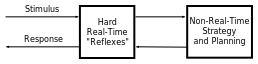
\includegraphics{advsync/rt-reflexes}}
\caption{Real-Time Reflexes}
\label{fig:advsync:Real-Time Reflexes}
\end{figure}

One approach is to recognize the fact that many real-time systems
resemble biological nervous systems, with responses ranging from
real-time reflexes to non-real-time strategizing and planning,
as depicted in
\cref{fig:advsync:Real-Time Reflexes}.
The hard real-time reflexes, which read from sensors and control
actuators, run real-time on a single CPU or on special-purpose hardware
such as an FPGA\@.
The non-real-time strategy and planning portion of the application runs
on the remaining CPUs.
Strategy and planning activities might include statistical analysis,
periodic calibration, user interface, supply-chain activities, and
preparation.
For an example of high-compute-load preparation activities, think back
to the veneer-peeling application discussed in
\pararef{sec:advsync:Real-World Real-Time Specifications}.
While one CPU is attending to the high-speed real-time computations
required to peel one log, the other CPUs might be analyzing the size
and shape of the next log in order to determine how to position the
next log so as to obtain the largest cylinder of high-quality wood.
It turns out that many applications have non-real-time and real-time
components~\cite{RobertBerry2008IBMSysJ}, so this approach can
often be used to allow traditional real-time analysis to be combined
with modern multicore hardware.

Another trivial approach is to shut off all but one hardware thread so as
to return to the settled mathematics of uniprocessor real-time
computing.
However, this approach gives up potential cost and energy-efficiency
advantages.
That said, obtaining these advantages requires overcoming the parallel
performance obstacles covered in
\cref{chp:Hardware and its Habits},
and not merely on average, but instead in the worst case.

Implementing parallel real-time systems can therefore be quite a
challenge.
Ways of meeting this challenge are outlined in the following section.

\subsection{Implementing Parallel Real-Time Systems}
\label{sec:advsync:Implementing Parallel Real-Time Systems}

We will look at two major styles of real-time systems, event-driven and
polling.
An event-driven real-time system remains idle much of the time, responding
in real time to events passed up through the operating system to the
application.
Alternatively, the system could instead be running a background
non-real-time workload.
A polling real-time system features a real-time thread that is CPU
bound, running in a tight loop that polls inputs and updates outputs on
each pass.
This tight polling loop often executes entirely in user mode, reading from
and writing to hardware registers that have been mapped into the user-mode
application's address space.
Alternatively, some applications place the polling loop into the kernel,
for example, using loadable kernel modules.

\begin{figure}
\centering
\resizebox{3in}{!}{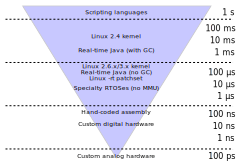
\includegraphics{advsync/rt-regimes}}
\caption{Real-Time Response Regimes}
\label{fig:advsync:Real-Time Response Regimes}
\end{figure}

Regardless of the style chosen, the approach used to implement a real-time
system will depend on the deadlines, for example, as shown in
\cref{fig:advsync:Real-Time Response Regimes}.
Starting from the top of this figure, if you can live with response times in
excess of one second, you might well be able to use scripting languages
to implement your real-time application---and scripting languages are
in fact used surprisingly often, not that I necessarily recommend this
practice.
If the required latencies exceed several tens of milliseconds,
old 2.4 versions of the Linux kernel can be used, not that I necessarily
recommend this practice, either.
Special real-time Java implementations can provide real-time response
latencies of a few milliseconds, even when the garbage collector is
used.
The Linux 2.6.x and 3.x kernels can provide real-time latencies of
a few hundred microseconds if carefully configured, tuned, and run
on real-time friendly hardware.
Special real-time Java implementations can provide real-time latencies
below 100 microseconds if use of the garbage collector is carefully avoided.
(But note that avoiding the garbage collector means also avoiding
Java's large standard libraries, thus also avoiding Java's productivity
advantages.)
The Linux 4.x and 5.x kernels can provide deep sub-hundred-millisecond
latencies, but with all the same caveats as for the 2.6.x and 3.x kernels.
A Linux kernel incorporating the \rt\ patchset can provide latencies
well below 20 microseconds, and specialty real-time operating systems (RTOSes)
running without MMUs can provide sub-ten-microsecond
latencies.
Achieving sub-microsecond latencies typically requires hand-coded assembly
or even special-purpose hardware.

Of course, careful configuration and tuning are required all the way down
the stack.
In particular, if the hardware or firmware fails to provide real-time
latencies, there is nothing that the software can do to make up for the
lost time.
Worse yet, high-performance hardware sometimes sacrifices worst-case behavior
to obtain greater throughput.
In fact, timings from tight loops run with interrupts disabled can
provide the basis for a high-quality random-number
generator~\cite{PeterOkech2009InherentRandomness}.
Furthermore, some firmware does cycle-stealing to carry out various
housekeeping tasks, in some cases attempting to cover its tracks by
reprogramming the victim CPU's hardware clocks.
Of course, cycle stealing is expected behavior in virtualized
environment, but people are nevertheless working towards real-time
response in virtualized
environments~\cite{ThomasGleixner2012KVMrealtime,JanKiszka2014virtRT}.
It is therefore critically important to evaluate your hardware's and
firmware's real-time capabilities.

But given competent real-time hardware and firmware, the next
layer up the stack is the operating system, which is covered in
the next section.

\subsection{Implementing Parallel Real-Time Operating Systems}
\label{sec:advsync:Implementing Parallel Real-Time Operating Systems}

\begin{figure}
\centering
\resizebox{2.2in}{!}{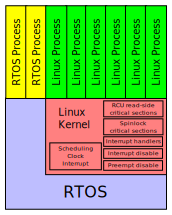
\includegraphics{advsync/Linux-on-RTOS}}
\caption{Linux Ported to RTOS}
\label{fig:advsync:Linux Ported to RTOS}
\end{figure}

There are a number of strategies that may be used to implement a
real-time system.
One approach is to port a general-purpose non-real-time OS on top
of a special purpose real-time operating system (RTOS), as shown in
\cref{fig:advsync:Linux Ported to RTOS}.
The green ``Linux Process'' boxes represent non-real-time processes
running on the Linux kernel, while the yellow ``RTOS Process''
boxes represent real-time processes running on the RTOS\@.

This was a very popular approach before the Linux kernel gained
real-time capabilities, and is still in
use~\cite{Xenomai2014,VictorYodaiken2004a}.
However, this approach requires that the application be split into
one portion that runs on the RTOS and another that runs on Linux.
Although it is possible to make the two environments look similar,
for example, by forwarding POSIX system calls from the RTOS to a
utility thread running on Linux, there are invariably rough edges.

In addition, the RTOS must interface to both the hardware and to
the Linux kernel, thus requiring significant maintenance with
changes in both hardware and kernel.
Furthermore, each such RTOS often has its own system-call interface
and set of system libraries, which can balkanize both ecosystems and
developers.
In fact, these problems seem to be what drove the combination of
RTOSes with Linux, as this approach allowed access to the full real-time
capabilities of the RTOS, while allowing the application's non-real-time
code full access to Linux's open-source ecosystem.

\begin{figure*}
\centering
\IfEbookSize{
\resizebox{.87\onecolumntextwidth}{!}{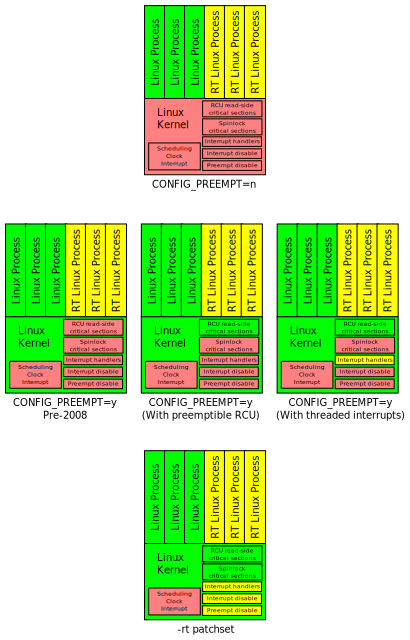
\includegraphics{advsync/preemption}}
}{
\resizebox{4.4in}{!}{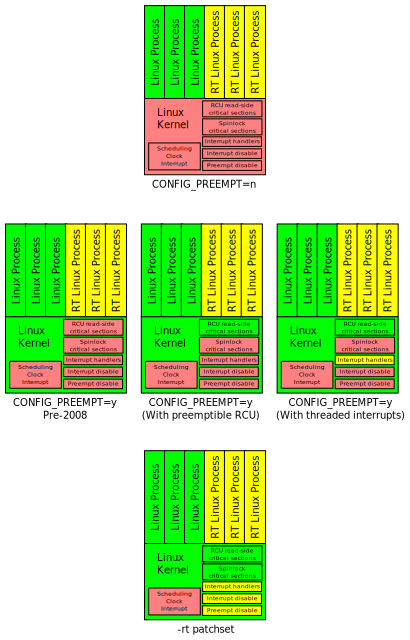
\includegraphics{advsync/preemption}}
}
\caption{Linux-Kernel Real-Time Implementations}
\label{fig:advsync:Linux-Kernel Real-Time Implementations}
\end{figure*}

Although pairing RTOSes with the Linux kernel was a clever and useful
short-term response during the time that the Linux kernel had minimal
real-time capabilities, it also motivated adding real-time capabilities
to the Linux kernel.
Progress towards this goal is shown in
\cref{fig:advsync:Linux-Kernel Real-Time Implementations}.
The upper row shows a diagram of the Linux kernel with preemption disabled,
thus having essentially no real-time capabilities.
The middle row shows a set of diagrams showing the increasing real-time
capabilities of the mainline Linux kernel with preemption enabled.
Finally, the bottom row shows a diagram of the Linux kernel with the
\rt\ patchset applied, maximizing real-time capabilities.
Functionality from the \rt\ patchset is added to mainline,
hence the increasing capabilities of the mainline Linux kernel over time.
Nevertheless, the most demanding real-time applications continue to use
the \rt\ patchset.

The non-preemptible kernel shown at the top of
\cref{fig:advsync:Linux-Kernel Real-Time Implementations}
is built with \co{CONFIG_PREEMPT=n}, so that execution within the Linux
kernel cannot be preempted.
This means that the kernel's real-time response latency is bounded below
by the longest code path in the Linux kernel, which is indeed long.
However, user-mode execution is preemptible, so that one of the
real-time Linux processes shown in the upper right may preempt any of the
non-real-time Linux processes shown in the upper left anytime the
non-real-time process is executing in user mode.

The middle row of
\cref{fig:advsync:Linux-Kernel Real-Time Implementations}
shows three stages (from left to right) in the development of Linux's
preemptible kernels.
In all three stages, most process-level code within the Linux kernel
can be preempted.
This of course greatly improves real-time response latency, but
preemption is still disabled
within RCU read-side critical sections,
spinlock critical sections,
interrupt handlers,
interrupt-disabled code regions, and
preempt-disabled code regions, as indicated by the red boxes in the
left-most diagram in the middle row of the figure.
The advent of preemptible RCU allowed RCU read-side critical sections
to be preempted, as shown in the central diagram,
and the advent of threaded interrupt handlers allowed device-interrupt
handlers to be preempted, as shown in the right-most diagram.
Of course, a great deal of other real-time functionality was added
during this time, however, it cannot be as easily represented on this
diagram.
It will instead be discussed in
\cref{sec:advsync:Event-Driven Real-Time Support}.

The bottom row of
\cref{fig:advsync:Linux-Kernel Real-Time Implementations}
shows the \rt\ patchset, which features threaded (and thus preemptible)
interrupt handlers for many devices, which also allows the corresponding
``interrupt-disabled'' regions of these drivers to be preempted.
These drivers instead use locking to coordinate the process-level
portions of each driver with its threaded interrupt handlers.
Finally, in some cases, disabling of preemption is replaced by
disabling of migration.
These measures result in excellent response times in many systems running
the \rt\ patchset~\cite{Reghenzani:2019:RLK:3309872.3297714,DanielBristot2019RTtrace}.

\begin{figure}
\centering
\resizebox{2.5in}{!}{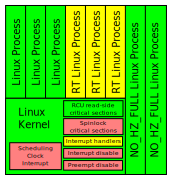
\includegraphics{advsync/nohzfull}}
\caption{CPU Isolation}
\label{fig:advsync:CPU Isolation}
\end{figure}

A final approach is simply to get everything out of the way of the
real-time process, clearing all other processing off of any CPUs that
this process needs, as shown in \cref{fig:advsync:CPU Isolation}.
This was implemented in the 3.10 Linux kernel via the \co{CONFIG_NO_HZ_FULL}
Kconfig parameter~\cite{JonCorbet2013NO-HZ-FULL,FredericWeisbecker2013nohz}.
It is important to note that this approach requires at least one
\emph{housekeeping CPU} to do background processing, for example running
kernel daemons.
However, when there is only one runnable task on a given non-housekeeping CPU,
scheduling-clock interrupts are shut off on that CPU, removing an important
source of interference and \emph{OS jitter}.
With a few exceptions, the kernel does not force other processing off of the
non-housekeeping CPUs, but instead simply provides better performance
when only one runnable task is present on a given CPU\@.
Any number of userspace tools may be used to force a given CPU to have
no more that one runnable task.
If configured properly, a non-trivial undertaking, \co{CONFIG_NO_HZ_FULL}
offers real-time threads levels of performance that come close to those of
bare-metal systems~\cite{AbdullahAljuhni2018nohzfull}.
\ppl{Fr\'{e}d\'{e}ric}{Weisbecker} produced a practical guide to
\co{CONFIG_NO_HZ_FULL} configuration~\cite{
	FredericWeisbecker2022nohzIntro,
	FredericWeisbecker2022nohzFullDynticksInternals,
	FredericWeisbecker2022nohzfull,
	FredericWeisbecker2022HousekeepingTradeoffs,
	FredericWeisbecker2022practicalExample,
	FredericWeisbecker2022nohzfullTSC}.

There has of course been much debate over which of these approaches
is best for real-time systems, and this debate has been going on for
quite some
time~\cite{JonCorbet2004RealTimeLinuxPart1,JonCorbet2004RealTimeLinuxPart2}.
As usual, the answer seems to be ``It depends,'' as discussed in the
following sections.
\Cref{sec:advsync:Event-Driven Real-Time Support}
considers event-driven real-time systems, and
\cref{sec:advsync:Polling-Loop Real-Time Support}
considers real-time systems that use a CPU-bound polling loop.

\subsubsection{Event-Driven Real-Time Support}
\label{sec:advsync:Event-Driven Real-Time Support}

The operating-system support required for event-driven real-time
applications is quite extensive, however, this section will focus
on only a few items, namely
timers,
threaded interrupts,
priority inheritance,
preemptible RCU,
and
preemptible spinlocks.

\paragraph{Timers} are clearly critically important for real-time
operations.
After all, if you cannot specify that something be done at a specific
time, how are you going to respond by that time?
Even in non-real-time systems, large numbers of timers are generated,
so they must be handled extremely efficiently.
Example uses include retransmit timers for TCP connections (which are
almost always canceled before they have a chance to fire),\footnote{
	At least assuming reasonably low packet-loss rates!}
timed delays (as in \co{sleep(1)}, which are rarely canceled),
and timeouts for the \co{poll()} system call (which are often
canceled before they have a chance to fire).
A good data structure for such timers would therefore be a priority queue
whose addition and deletion primitives were fast and $\O{1}$ in the number
of timers posted.

The classic data structure for this purpose is the \emph{calendar queue},
which in the Linux kernel is called the \co{timer wheel}.
This age-old data structure is also heavily used in discrete-event
simulation.
The idea is that time is quantized, for example, in the Linux kernel,
the duration of the time quantum is the period of the scheduling-clock
interrupt.
A given time can be represented by an integer, and any attempt to post
a timer at some non-integral time will be rounded to a convenient nearby
integral time quantum.

One straightforward implementation would be to allocate a single array,
indexed by the low-order bits of the time.
This works in theory, but in practice systems create large numbers of
long-duration timeouts (for example, the two-hour keepalive timeouts for TCP
sessions) that are almost always canceled.
These long-duration timeouts cause problems for small arrays because
much time is wasted skipping timeouts that have not yet expired.
On the other hand, an array that is large enough to gracefully accommodate
a large number of long-duration timeouts would consume too much memory,
especially given that performance and scalability concerns require one
such array for each and every CPU\@.

\begin{figure}
\centering
\resizebox{2.0in}{!}{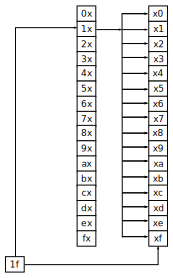
\includegraphics{advsync/timerwheel}}
\caption{Timer Wheel}
\label{fig:advsync:Timer Wheel}
\end{figure}

A common approach for resolving this conflict is to provide multiple
arrays in a hierarchy.
At the lowest level of this hierarchy, each array element represents
one unit of time.
At the second level, each array element represents $N$ units of time,
where $N$ is the number of elements in each array.
At the third level, each array element represents $N^2$ units of time,
and so on up the hierarchy.
This approach allows the individual arrays to be indexed by different
bits, as illustrated by
\cref{fig:advsync:Timer Wheel}
for an unrealistically small eight-bit clock.
Here, each array has 16 elements, so the low-order four bits of the time
(currently \co{0xf}) index the low-order (rightmost) array, and the
next four bits (currently \co{0x1}) index the next level up.
Thus, we have two arrays each with 16 elements, for a total of 32 elements,
which, taken together, is much smaller than the 256-element array that
would be required for a single array.

This approach works extremely well for throughput-based systems.
Each timer operation is $\O{1}$ with small constant, and each timer
element is touched at most $m+1$ times, where $m$ is the number of
levels.

\begin{figure}
\centering
\resizebox{3.0in}{!}{\includegraphics{cartoons/1kHz}}
\caption{Timer Wheel at 1\,kHz}
\ContributedBy{Figure}{fig:advsync:Timer Wheel at 1kHz}{Melissa Broussard}
\end{figure}

\begin{figure}
\centering
\resizebox{3.0in}{!}{\includegraphics{cartoons/100kHz}}
\caption{Timer Wheel at 100\,kHz}
\ContributedBy{Figure}{fig:advsync:Timer Wheel at 100kHz}{Melissa Broussard}
\end{figure}

Unfortunately, timer wheels do not work well for real-time systems, and for
two reasons.
The first reason is that there is a harsh tradeoff between timer
accuracy and timer overhead, which is fancifully illustrated by
\cref{fig:advsync:Timer Wheel at 1kHz,fig:advsync:Timer Wheel at 100kHz}.
In \cref{fig:advsync:Timer Wheel at 1kHz},
timer processing happens only once per millisecond, which keeps overhead
acceptably low for many (but not all!\@) workloads, but which also means
that timeouts cannot be set for finer than one-millisecond granularities.
On the other hand, \cref{fig:advsync:Timer Wheel at 100kHz}
shows timer processing taking place every ten microseconds, which
provides acceptably fine timer granularity for most (but not all!\@)
workloads, but which processes timers so frequently that the system
might well not have time to do anything else.

The second reason is the need to cascade timers from higher levels to
lower levels.
Referring back to \cref{fig:advsync:Timer Wheel},
we can see that any timers enqueued on element \co{1x} in the upper
(leftmost) array must be cascaded down to the lower (rightmost)
array so that may be invoked when their time arrives.
Unfortunately, there could be a large number of timeouts
waiting to be cascaded, especially for timer wheels with larger numbers
of levels.
The power of statistics causes this cascading to be a non-problem for
throughput-oriented systems, but cascading can result in problematic
degradations of latency in real-time systems.

\IfTwoColumn{
\begin{figure*}
\centering
\resizebox{1.4\twocolumnwidth}{!}{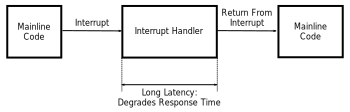
\includegraphics{advsync/irq}}
\caption{Non-Threaded Interrupt Handler}
\label{fig:advsync:Non-Threaded Interrupt Handler}
\end{figure*}
}{}

\IfTwoColumn{
\begin{figure*}
\centering
\resizebox{1.4\twocolumnwidth}{!}{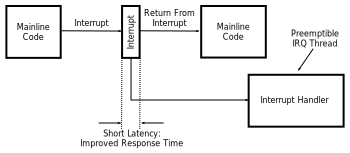
\includegraphics{advsync/threaded-irq}}
\caption{Threaded Interrupt Handler}
\label{fig:advsync:Threaded Interrupt Handler}
\end{figure*}
}{}

Of course, real-time systems could simply choose a different data
structure, for example, some form of heap or tree, giving up
$\O{1}$ bounds on insertion and deletion operations to gain $\O{\log n}$
limits on data-structure-maintenance operations.
This can be a good choice for special-purpose RTOSes, but is inefficient
for general-purpose systems such as Linux, which routinely support
extremely large numbers of timers.

The solution chosen for the Linux kernel's \rt\ patchset is to differentiate
between timers that schedule later activity and timeouts that schedule
error handling for low-probability errors such as TCP packet losses.
One key observation is that error handling is normally not particularly
time-critical, so that a timer wheel's millisecond-level granularity
is good and sufficient.
Another key observation is that error-handling timeouts are normally
canceled very early, often before they can be cascaded.
In addition, systems commonly have many more error-handling timeouts
than they do timer events, so that an $\O{\log n}$ data structure should
provide acceptable performance for timer events.

However, it is possible to do better, namely by simply refusing to
cascade timers.
Instead of cascading, the timers that would otherwise have been cascaded
all the way down the calendar queue are handled in place.
This does result in up to a few percent error for the time duration,
but the few situations where this is a problem can instead use tree-based
high-resolution timers (hrtimers).

In short, the Linux kernel's \rt\ patchset uses timer wheels for
error-handling timeouts and a tree for timer events, providing each
category the required quality of service.

\IfTwoColumn{}{
\begin{figure}
\centering
\IfEbookSize{
\resizebox{\onecolumntextwidth}{!}{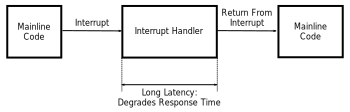
\includegraphics{advsync/irq}}
}{
\resizebox{1.4\twocolumnwidth}{!}{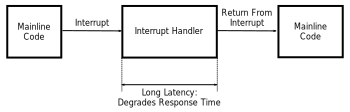
\includegraphics{advsync/irq}}
}
\caption{Non-Threaded Interrupt Handler}
\label{fig:advsync:Non-Threaded Interrupt Handler}
\end{figure}
}

\paragraph{Threaded interrupts}
are used to address a significant source of degraded real-time latencies,
namely long-running interrupt handlers,
as shown in \cref{fig:advsync:Non-Threaded Interrupt Handler}.
These latencies can be especially problematic for devices that can
deliver a large number of events with a single interrupt, which means
that the interrupt handler will run for an extended period of time
processing all of these events.
Worse yet are devices that can deliver new events to a still-running
interrupt handler, as such an interrupt handler might well run
indefinitely, thus indefinitely degrading real-time latencies.

\IfTwoColumn{}{
\begin{figure}
\centering
\IfEbookSize{
\resizebox{\onecolumntextwidth}{!}{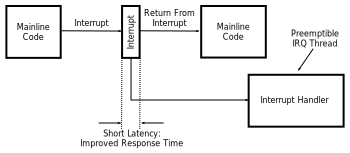
\includegraphics{advsync/threaded-irq}}
}{
\resizebox{1.4\twocolumnwidth}{!}{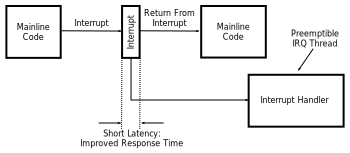
\includegraphics{advsync/threaded-irq}}
}
\caption{Threaded Interrupt Handler}
\label{fig:advsync:Threaded Interrupt Handler}
\end{figure}
}

One way of addressing this problem is the use of threaded interrupts shown in
\cref{fig:advsync:Threaded Interrupt Handler}.
Interrupt handlers run in the context of a preemptible \IXacr{irq} thread,
which runs at a configurable priority.
The device interrupt handler then runs for only a short time, just
long enough to make the \IRQ\ thread aware of the new event.
As shown in the figure, threaded interrupts can greatly improve
real-time latencies, in part because interrupt handlers running in
the context of the \IRQ\ thread may be preempted by high-priority real-time
threads.

However, there is no such thing as a free lunch, and there are downsides
to threaded interrupts.
One downside is increased interrupt latency.
Instead of immediately running the interrupt handler, the handler's execution
is deferred until the \IRQ\ thread gets around to running it.
Of course, this is not a problem unless the device generating the interrupt
is on the real-time application's critical path.

Another downside is that poorly written high-priority real-time code
might starve the interrupt handler, for example, preventing networking
code from running, in turn making it very difficult to debug the problem.
Developers must therefore take great care when writing high-priority
real-time code.
This has been dubbed the \emph{Spiderman principle}:
With great power comes great responsibility.

\paragraph{Priority inheritance} is used to handle priority inversion,
which can be caused by, among other things, locks acquired by
preemptible interrupt handlers~\cite{LuiSha1990PriorityInheritance}.
Suppose that a low-priority thread holds a lock, but is preempted by
a group of medium-priority threads, at least one such thread per CPU\@.
If an interrupt occurs, a high-priority \IRQ\ thread will preempt one
of the medium-priority threads, but only until it decides to acquire
the lock held by the low-priority thread.
Unfortunately, the low-priority thread cannot release the lock until
it starts running, which the medium-priority threads prevent it from
doing.
So the high-priority \IRQ\ thread cannot acquire the lock until after one
of the medium-priority threads releases its CPU\@.
In short, the medium-priority threads are indirectly blocking the
high-priority \IRQ\ threads, a classic case of priority inversion.

Note that this priority inversion could not happen with non-threaded
interrupts because the low-priority thread would have to disable interrupts
while holding the lock, which would prevent the medium-priority
threads from preempting it.

In the priority-inheritance solution, the high-priority thread attempting
to acquire the lock donates its priority to the low-priority thread holding
the lock until such time as the lock is released, thus preventing long-term
priority inversion.

\begin{figure}
\centering
\resizebox{3.4in}{!}{\includegraphics{cartoons/Priority_Boost_2}}
\caption{Priority Inversion and User Input}
\ContributedBy{Figure}{fig:advsync:Priority Inversion and User Input}{Melissa Broussard}
\end{figure}

Of course, priority inheritance does have its limitations.
For example, if you can design your application to avoid priority
inversion entirely, you will likely obtain somewhat better
latencies~\cite{VictorYodaiken2004a}.
This should be no surprise, given that priority inheritance adds
a pair of context switches to the worst-case latency.
That said, priority inheritance can convert indefinite postponement
into a limited increase in latency, and the software-engineering
benefits of priority inheritance may outweigh its latency costs in
many applications.

Another limitation is that it addresses only lock-based priority
inversions within the context of a given operating system.
One priority-inversion scenario that it cannot address is a high-priority
thread waiting on a network socket for a message that is to be written
by a low-priority process that is preempted by a set of CPU-bound
medium-priority processes.
In addition, a potential disadvantage of applying priority inheritance
to user input is fancifully depicted in
\cref{fig:advsync:Priority Inversion and User Input}.

A final limitation involves reader-writer locking.
Suppose that we have a very large number of low-priority threads, perhaps
even thousands of them, each
of which read-holds a particular reader-writer lock.
Suppose that all of these threads are preempted by a set of medium-priority
threads, with at least one medium-priority thread per CPU\@.
Finally, suppose that a high-priority thread awakens and attempts to
write-acquire this same reader-writer lock.
No matter how vigorously we boost the priority of the threads read-holding
this lock, it could well be a good long time before the high-priority
thread can complete its write-acquisition.

There are a number of possible solutions to this reader-writer lock
priority-inversion conundrum:

\begin{enumerate}
\item	Only allow one read-acquisition of a given reader-writer lock
	at a time.
	(This is the approach traditionally taken by the Linux
	kernel's \rt\ patchset.)
\item	Only allow $N$ read-acquisitions of a given reader-writer lock
	at a time, where $N$ is the number of CPUs.
\item	Only allow $N$ read-acquisitions of a given reader-writer lock
	at a time, where $N$ is a number specified somehow by the
	developer.
\item	Prohibit high-priority threads from write-acquiring reader-writer
	locks that are ever read-acquired by threads running at lower
	priorities.
	(This is a variant of the \emph{priority ceiling}
	protocol~\cite{LuiSha1990PriorityInheritance}.)
\end{enumerate}

\QuickQuiz{
	But if you only allow one reader at a time to read-acquire
	a reader-writer lock, isn't that the same as an exclusive
	lock???
}\QuickQuizAnswer{
	Indeed it is, other than the API\@.
	And the API is important because it allows the Linux kernel
	to offer real-time capabilities without having the \rt\ patchset
	grow to ridiculous sizes.

	However, this approach clearly and severely limits read-side
	scalability.
	The Linux kernel's \rt\ patchset was long able to live with this
	limitation for several reasons:
	\begin{enumerate*}[(1)]
	\item Real-time systems have traditionally been relatively small,
	\item Real-time systems have generally focused on process control,
	thus being unaffected by scalability limitations in the
	I/O subsystems, and
	\item Many of the Linux kernel's reader-writer locks have been
	converted to RCU\@.
	\end{enumerate*}

	However, the day came when it was absolutely necessary to
	permit concurrent readers, as described in the text following
	this quiz.
}\QuickQuizEnd

The no-concurrent-readers restriction eventually became intolerable, so
the \rt\ developers looked more carefully at how the Linux kernel uses
reader-writer spinlocks.
They learned that time-critical code rarely uses those parts of the
kernel that write-acquire reader-writer locks, so that the prospect
of writer \IX{starvation} was not a show-stopper.
They therefore constructed a real-time reader-writer lock in which
write-side acquisitions use priority inheritance among each other,
but where read-side acquisitions take absolute priority over
write-side acquisitions.
This approach appears to be working well in practice, and is another
lesson in the importance of clearly understanding what your users
really need.

One interesting detail of this implementation is that both the
\co{rt_read_lock()} and the \co{rt_write_lock()} functions enter an RCU
read-side critical section and both the \co{rt_read_unlock()} and the
\co{rt_write_unlock()} functions exit that critical section.
This is necessary because non-realtime kernels' reader-writer locking
functions disable preemption across their critical sections, and
there really are reader-writer locking use cases that rely on the fact
that \co{synchronize_rcu()} will therefore wait for all pre-exiting
reader-writer-lock critical sections to complete.
Let this be a lesson to you:
Understanding what your users really need is critically important to
correct operation, not just to performance.
Not only that, but what your users really need changes over time.

This has the side-effect that all of a \rt\ kernel's reader-writer locking
critical sections are subject to RCU priority boosting.
This provides at least a partial solution to the problem of reader-writer
lock readers being preempted for extended periods of time.

It is also possible to avoid reader-writer lock priority inversion by
converting the reader-writer lock to RCU, as briefly discussed in the
next section.

\paragraph{Preemptible RCU}
can sometimes be used as a replacement for reader-writer
locking~\cite{PaulEMcKenney2007WhatIsRCUFundamentally,PaulMcKenney2012RCUUsage,PaulEMcKenney2014RCUAPI},
as was discussed in \cref{sec:defer:Read-Copy Update (RCU)}.
Where it can be used, it permits readers and updaters to run concurrently,
which prevents low-priority readers from inflicting any sort of
priority-inversion scenario on high-priority updaters.
However, for this to be useful, it is necessary to be able to preempt
long-running RCU read-side critical
sections~\cite{DinakarGuniguntala2008IBMSysJ}.
Otherwise, long RCU read-side critical sections would result in
excessive real-time latencies.

\begin{listing}
\begin{fcvlabel}[ln:advsync:Preemptible Linux-Kernel RCU]
\begin{VerbatimL}[commandchars=\\\[\]]
void __rcu_read_lock(void)			\lnlbl[lock:b]
{
	current->rcu_read_lock_nesting++;	\lnlbl[lock:inc]
	barrier();				\lnlbl[lock:bar]
}						\lnlbl[lock:e]

void __rcu_read_unlock(void)		        \lnlbl[unl:b]
{
	barrier();				\lnlbl[unl:bar1]
	if (!--current->rcu_read_lock_nesting)	\lnlbl[unl:decchk]
		barrier();			\lnlbl[unl:bar2]
		if (READ_ONCE(current->rcu_read_unlock_special.s)) { \lnlbl[unl:chks]
			rcu_read_unlock_special(t); \lnlbl[unl:unls]
		}				\lnlbl[unl:if:e]
}						\lnlbl[unl:e]
\end{VerbatimL}
\end{fcvlabel}
\caption{Preemptible Linux-Kernel RCU}
\label{lst:advsync:Preemptible Linux-Kernel RCU}
\end{listing}

A preemptible RCU implementation was therefore added to the Linux kernel.
This implementation avoids the need to individually track the state of
each and every task in the kernel by keeping lists of tasks that have
been preempted within their current RCU read-side critical sections.
A \IX{grace period} is permitted to end:
\begin{enumerate*}[(1)]
\item Once all CPUs have completed any RCU read-side critical sections
that were in effect before the start of the current grace period and
\item Once all tasks that were preempted
while in one of those pre-existing critical sections have removed
themselves from their lists.
\end{enumerate*}
A simplified version of this implementation is shown in
\cref{lst:advsync:Preemptible Linux-Kernel RCU}.
\begin{fcvref}[ln:advsync:Preemptible Linux-Kernel RCU]
The \co{__rcu_read_lock()} function spans \clnrefrange{lock:b}{lock:e} and
the \co{__rcu_read_unlock()} function spans \clnrefrange{unl:b}{unl:e}.
\end{fcvref}

\begin{fcvref}[ln:advsync:Preemptible Linux-Kernel RCU:lock]
\Clnref{inc} of \co{__rcu_read_lock()} increments a per-task count of the
number of nested \co{rcu_read_lock()} calls, and
\clnref{bar} prevents the compiler from reordering the subsequent code in the
RCU read-side critical section to precede the \co{rcu_read_lock()}.
\end{fcvref}

\begin{fcvref}[ln:advsync:Preemptible Linux-Kernel RCU:unl]
\Clnref{bar1} of \co{__rcu_read_unlock()} prevents the compiler from
reordering the code in the critical section with the remainder of
this function.
\Clnref{decchk} decrements the nesting count and checks to see if it
has become zero, in other words, if this corresponds to the outermost
\co{rcu_read_unlock()} of a nested set.
If so, \clnref{bar2} prevents the compiler from reordering this nesting
update with \clnref{chks}'s check for special handling.
If special handling is required, then the call to
\co{rcu_read_unlock_special()} on \clnref{unls} carries it out.

There are several types of special handling that can be required, but
we will focus on that required when the RCU read-side critical section
has been preempted.
In this case, the task must remove itself from the list that it was
added to when it was first preempted within its
RCU read-side critical section.
However, it is important to note that these lists are protected by locks,
which means that \co{rcu_read_unlock()} is no longer lockless.
However, the highest-priority threads will not be preempted, and therefore,
for those highest-priority threads, \co{rcu_read_unlock()} will never
attempt to acquire any locks.
In addition, if implemented carefully, locking can be used to synchronize
real-time software~\cite{BjoernBrandenburgPhD,DipankarSarma2004OLSscalability}.
\end{fcvref}

\QuickQuiz{
	\begin{fcvref}[ln:advsync:Preemptible Linux-Kernel RCU:unl]
	Suppose that preemption occurs just after the load from
	\co{t->rcu_read_unlock_special.s} on \clnref{chks} of
	\cref{lst:advsync:Preemptible Linux-Kernel RCU}.
	Mightn't that result in the task failing to invoke
	\co{rcu_read_unlock_special()}, thus failing to remove itself
	from the list of tasks blocking the current grace period,
	in turn causing that grace period to extend indefinitely?
	\end{fcvref}
}\QuickQuizAnswer{
	That is a real problem, and it is solved in RCU's scheduler hook.
	If that scheduler hook sees that the value of
	\co{t->rcu_read_lock_nesting} is negative, it invokes
	\co{rcu_read_unlock_special()} if needed before allowing
	the context switch to complete.
}\QuickQuizEnd

Another important real-time feature of RCU, whether preemptible or
not, is the ability to offload RCU callback execution to a kernel
thread.
To use this, your kernel must be built with \co{CONFIG_RCU_NOCB_CPU=y}
and booted with the \co{rcu_nocbs=} kernel boot parameter specifying
which CPUs are to be offloaded.
Alternatively, any CPU specified by the \co{nohz_full=} kernel boot parameter
described in
\cref{sec:advsync:Polling-Loop Real-Time Support}
will also have its RCU callbacks offloaded.

In short, this preemptible RCU implementation enables real-time response for
read-mostly data structures without the delays inherent to priority
boosting of large numbers of readers, and also without delays due to
callback invocation.

\paragraph{Preemptible spinlocks}
are an important part of the \rt\ patchset due to the long-duration
spinlock-based critical sections in the Linux kernel.
This functionality has not yet reached mainline:
Although they are a conceptually simple substitution of sleeplocks
for spinlocks, they have proven relatively controversial.
In addition the real-time functionality that is already in the mainline
Linux kernel suffices for a great many use cases, which slowed the \rt\
patchset's development rate in the early
2010s~\cite{JakeEdge2013Future-rtLinux,JakeEdge2014Future-rtLinux}.
However, preemptible spinlocks are absolutely necessary to the task of
achieving real-time latencies down in the tens of microseconds.
Fortunately, Linux Foundation organized an effort to fund moving the
remaining code from the \rt\ patchset to mainline.

\paragraph{Per-CPU variables}\ are used heavily in the Linux kernel
for performance reasons.
Unfortunately for real-time applications, many use cases for per-CPU
variables require coordinated update of multiple such variables,
which is normally provided by disabling preemption, which in turn
degrades real-time latencies.
Real-time applications clearly need some other way of coordinating
per-CPU variable updates.

One alternative is to supply per-CPU spinlocks, which as noted above
are actually sleeplocks, so that their critical sections can be
preempted and so that priority inheritance is provided.
In this approach, code updating groups of per-CPU variables must
acquire the current CPU's spinlock, carry out the update, then
release whichever lock is acquired, keeping in mind that a preemption
might have resulted in a migration to some other CPU\@.
However, this approach introduces both overhead and \IXpl{deadlock}.

Another alternative, which is used in the \rt\ patchset as of early 2021,
is to convert preemption disabling to migration disabling.
This ensures that a given kernel thread remains on its CPU through
the duration of the per-CPU-variable update, but could also allow some
other kernel thread to intersperse its own update of those same variables,
courtesy of preemption.
There are cases such as statistics gathering where this is not a problem.
In the surprisingly rare case where such mid-update preemption is a problem,
the use case at hand must properly synchronize the updates, perhaps through
a set of per-CPU locks specific to that use case.
Although introducing locks again introduces the possibility of deadlock,
the per-use-case nature of these locks makes any such deadlocks easier
to manage and avoid.

\paragraph{Closing event-driven remarks.}
There are of course any number of other Linux-kernel components that are
critically important to achieving world-class real-time latencies,
for example, deadline
scheduling~\cite{DanielBristot2018deadlinesched-1,DanielBristot2018deadlinesched-2},
however, those listed in this section give a good feeling for the workings
of the Linux kernel augmented by the \rt\ patchset.

\subsubsection{Polling-Loop Real-Time Support}
\label{sec:advsync:Polling-Loop Real-Time Support}

At first glance, use of a polling loop might seem to avoid all possible
operating-system interference problems.
After all, if a given CPU never enters the kernel, the kernel is
completely out of the picture.
And the traditional approach to keeping the kernel out of the way is
simply not to have a kernel, and many real-time applications do
indeed run on bare metal, particularly those running on eight-bit
microcontrollers.

One might hope to get bare-metal performance on a modern operating-system
kernel simply by running a single CPU-bound user-mode thread on a
given CPU, avoiding all causes of interference.
Although the reality is of course more complex, it is becoming
possible to do just that,
courtesy of the \co{NO_HZ_FULL} implementation led by
Frederic Weisbecker~\cite{JonCorbet2013NO-HZ-FULL,FredericWeisbecker2013nohz}
that was accepted into version 3.10 of the Linux kernel.
Nevertheless, considerable care is required to properly set up such
an environment, as it is necessary to control a number of possible
sources of OS jitter.
The discussion below covers the control of several sources of OS
jitter, including device interrupts, kernel threads and daemons,
scheduler real-time throttling (this is a feature, not a bug!),
timers, non-real-time device drivers, in-kernel global synchronization,
scheduling-clock interrupts, page faults, and finally, non-real-time
hardware and firmware.

Interrupts are an excellent source of large amounts of OS jitter.
Unfortunately, in most cases interrupts are absolutely required in order
for the system to communicate with the outside world.
One way of resolving this conflict between OS jitter and maintaining
contact with the outside world is to reserve a small number of
housekeeping CPUs, and to force all interrupts to these CPUs.
The \path{Documentation/IRQ-affinity.txt} file in the Linux source tree
describes how to direct device interrupts to specified CPUs,
which as of early 2021 involves something like the following:

\begin{VerbatimU}
$ echo 0f > /proc/irq/44/smp_affinity
\end{VerbatimU}

This command would confine interrupt \#44 to CPUs~0--3.
Note that scheduling-clock interrupts require special handling, and are
discussed later in this section.

A second source of OS jitter is due to kernel threads and daemons.
Individual kernel threads, such as RCU's grace-period kthreads
(\co{rcu_bh}, \co{rcu_preempt}, and \co{rcu_sched}), may be forced
onto any desired CPUs using the \co{taskset} command, the
\co{sched_setaffinity()} system call, or \co{cgroups}.

Per-CPU kthreads are often more challenging, sometimes constraining
hardware configuration and workload layout.
Preventing OS jitter from these kthreads requires either that certain
types of hardware
not be attached to real-time systems, that all interrupts and I/O
initiation take place on housekeeping CPUs, that special kernel
Kconfig or boot parameters be selected in order to direct work away from
the worker CPUs, or that worker CPUs never enter the kernel.
Specific per-kthread advice may be found in the Linux kernel source
\path{Documentation} directory at \path{kernel-per-CPU-kthreads.txt}.

A third source of OS jitter in the Linux kernel for CPU-bound threads
running at real-time priority is the scheduler itself.
This is an intentional debugging feature, designed to ensure that
important non-realtime work is allotted at least 50 milliseconds
out of each second, even if there is an infinite-loop bug in
your real-time application.
However, when you are running a polling-loop-style real-time application,
you will need to disable this debugging feature.
This can be done as follows:

\begin{VerbatimU}
$ echo -1 > /proc/sys/kernel/sched_rt_runtime_us
\end{VerbatimU}

You will of course need to be running as root to execute this command,
and you will also need to carefully consider the aforementioned Spiderman
principle.
One way to minimize the risks is to offload interrupts and
kernel threads/daemons from all CPUs running CPU-bound real-time
threads, as described in the paragraphs above.
In addition, you should carefully read the material in the
\path{Documentation/scheduler} directory.
The material in the \path{sched-rt-group.rst} file is particularly
important, especially if you are using the \co{cgroups} real-time features
enabled by the \co{CONFIG_RT_GROUP_SCHED} Kconfig parameter.

A fourth source of OS jitter comes from timers.
In most cases, keeping a given CPU out of the kernel will prevent
timers from being scheduled on that CPU\@.
One important exception are recurring timers, where a given timer
handler posts a later occurrence of that same timer.
If such a timer gets started on a given CPU for any reason, that
timer will continue to run periodically on that CPU, inflicting
OS jitter indefinitely.
One crude but effective way to offload recurring timers is to
use CPU hotplug to offline all worker CPUs that are to run CPU-bound
real-time application threads, online these same CPUs, then start
your real-time application.

A fifth source of OS jitter is provided by device drivers that were
not intended for real-time use.
For an old canonical example, in 2005, the VGA driver would blank
the screen by zeroing the frame buffer with interrupts disabled,
which resulted in tens of milliseconds of OS jitter.
One way of avoiding device-driver-induced OS jitter is to carefully
select devices that have been used heavily in real-time systems,
and which have therefore had their real-time bugs fixed.
Another way is to confine the device's interrupts and all code using
that device to designated housekeeping CPUs.
A third way is to test the device's ability to support real-time
workloads and fix any real-time bugs.\footnote{
	If you take this approach, please submit your fixes upstream
	so that others can benefit.
	After all, when you need to port your application to
	a later version of the Linux kernel, \emph{you} will be one of those
	``others''.}

A sixth source of OS jitter is provided by some in-kernel
full-system synchronization algorithms, perhaps most notably
the global TLB-flush algorithm.
This can be avoided by avoiding memory-unmapping operations, and especially
avoiding unmapping operations within the kernel.
As of early 2021, the way to avoid in-kernel
unmapping operations is to avoid unloading kernel modules.

A seventh source of OS jitter is provided by
scheduling-clock interrrupts and RCU callback invocation.
These may be avoided by building your kernel with the
\co{NO_HZ_FULL} Kconfig parameter enabled, and then booting
with the \co{nohz_full=} parameter specifying the list of
worker CPUs that are to run real-time threads.
For example, \co{nohz_full=2-7} would designate CPUs~2, 3, 4, 5, 6, and~7
as worker CPUs, thus leaving CPUs~0 and~1 as housekeeping CPUs.
The worker CPUs would not incur scheduling-clock interrupts as long
as there is no more than one runnable task on each worker CPU,
and each worker CPU's RCU callbacks would be invoked on one of the
housekeeping CPUs.
A CPU that has suppressed scheduling-clock interrupts due to there
only being one runnable task on that CPU is said to be in
\emph{adaptive ticks mode} or in \co{nohz_full} mode.
It is important to ensure that you have designated enough
housekeeping CPUs to handle the housekeeping load imposed by the
rest of the system, which requires careful benchmarking and tuning.

An eighth source of OS jitter is page faults.
Because most Linux implementations use an MMU for memory protection,
real-time applications running on these systems can be subject
to page faults.
Use the \co{mlock()} and \co{mlockall()} system calls to pin your
application's pages into memory, thus avoiding major page faults.
Of course, the Spiderman principle applies, because locking down
too much memory may prevent the system from getting other work done.

A ninth source of OS jitter is unfortunately the hardware and firmware.
It is therefore important to use systems that have been designed for
real-time use.

\begin{listing}
\begin{fcvlabel}[ln:advsync:Locating Sources of OS Jitter]
\begin{VerbatimL}[commandchars=\\\[\]]
cd /sys/kernel/debug/tracing
echo 1 > max_graph_depth		\lnlbl[echo1]
echo function_graph > current_tracer
# run workload
cat per_cpu/cpuN/trace			\lnlbl[cat]
\end{VerbatimL}
\end{fcvlabel}
\caption{Locating Sources of OS Jitter}
\label{lst:advsync:Locating Sources of OS Jitter}
\end{listing}

\begin{fcvref}[ln:advsync:Locating Sources of OS Jitter]
Unfortunately, this list of OS-jitter sources can never be complete,
as it will change with each new version of the kernel.
This makes it necessary to be able to track down additional sources
of OS jitter.
Given a CPU $N$ running a CPU-bound usermode thread, the
commands shown in
\cref{lst:advsync:Locating Sources of OS Jitter}
will produce a list of all the times that this CPU entered the kernel.
Of course, the \co{N} on \clnref{cat} must be replaced with the
number of the CPU in question, and the \co{1} on \clnref{echo1} may be
increased
to show additional levels of function call within the kernel.
The resulting trace can help track down the source of the OS jitter.
\end{fcvref}

As always, there is no free lunch, and \co{NO_HZ_FULL} is no exception.
As noted earlier,
\co{NO_HZ_FULL} makes kernel/user transitions more expensive due to the
need for delta process accounting and the need to inform kernel subsystems
(such as RCU) of the transitions.
As a rough rule of thumb, \co{NO_HZ_FULL} helps with many types of
real-time and heavy-compute workloads, but hurts other workloads
that feature high rates of system calls and
I/O~\cite{AbdullahAljuhni2018nohzfull}.
Additional limitations, tradeoffs, and configuration advice may be
found in \path{Documentation/timers/no_hz.rst}.

As you can see, obtaining bare-metal performance when running
CPU-bound real-time threads on a general-purpose OS such as Linux
requires painstaking attention to detail.
Automation would of course help, and some automation has been applied,
but given the relatively small number of users, automation can be
expected to appear relatively slowly.
Nevertheless, the ability to gain near-bare-metal performance while
running a general-purpose operating system promises to ease construction
of some types of real-time systems.

\subsection{Implementing Parallel Real-Time Applications}
\label{sec:advsync:Implementing Parallel Real-Time Applications}

Developing real-time applications is a wide-ranging topic, and this
section can only touch on a few aspects.
To this end,
\cref{sec:advsync:Real-Time Components}
looks at a few software components commonly used in real-time applications,
\cref{sec:advsync:Polling-Loop Applications}
provides a brief overview of how polling-loop-based applications may
be implemented,
\cref{sec:advsync:Streaming Applications}
gives a similar overview of streaming applications, and
\cref{sec:advsync:Event-Driven Applications}
briefly covers event-based applications.

\subsubsection{Real-Time Components}
\label{sec:advsync:Real-Time Components}

As in all areas of engineering, a robust set of components is essential
to \IX{productivity} and \IX{reliability}.
This section is not a full catalog of real-time software components---such
a catalog would fill multiple books---but rather a brief overview of the
types of components available.

A natural place to look for real-time software components would be
algorithms offering wait-free
synchronization~\cite{Herlihy91}, and in fact lockless
algorithms are very important to real-time computing.
However, wait-free synchronization only guarantees forward progress in
finite time.
Although a century is finite, this is unhelpful when your deadlines are
measured in microseconds, let alone milliseconds.

Nevertheless, there are some important wait-free algorithms that do
provide bounded response time, including atomic test and set,
atomic exchange,
atomic fetch-and-add,
single-producer/single-consumer FIFO queues based on circular arrays,
and numerous per-thread partitioned algorithms.
In addition, recent research has confirmed the observation that
algorithms with lock-free guarantees\footnote{
	Wait-free algorithms guarantee that all threads make progress in
	finite time, while lock-free algorithms only guarantee that at
	least one thread will make progress in finite time.
	See \cref{sec:advsync:Non-Blocking Synchronization} for more details.}
also provide the same latencies in practice (in the wait-free sense),
assuming a stochastically fair scheduler and absence of fail-stop
bugs~\cite{DanAlitarh2013PracticalProgress}.
This means that many non-wait-free stacks and queues are nevertheless
appropriate for real-time use.

\QuickQuiz{
	But isn't correct operation despite fail-stop bugs
	a valuable fault-tolerance property?
}\QuickQuizAnswer{
	Yes and no.

	Yes in that non-blocking algorithms can provide fault tolerance
	in the face of fail-stop bugs, but no in that this is grossly
	insufficient for practical fault tolerance.
	For example, suppose you had a wait-free queue, and further
	suppose that a thread has just dequeued an element.
	If that thread now succumbs to a fail-stop bug, the element
	it has just dequeued is effectively lost.
	True fault tolerance requires way more than mere non-blocking
	properties, and is beyond the scope of this book.
}\QuickQuizEnd

In practice, locking is often used in real-time programs, theoretical
concerns notwithstanding.
However, under more severe constraints, lock-based
algorithms can also provide bounded latencies~\cite{BjoernBrandenburgPhD}.
These constraints include:

\begin{enumerate}
\item	Fair scheduler.
	In the common case of a fixed-priority scheduler, the bounded
	latencies are provided only to the highest-priority threads.
\item	Sufficient bandwidth to support the workload.
	An implementation rule supporting this constraint might be
	``There will be at least 50\,\% idle time on all CPUs
	during normal operation,''
	or, more formally, ``The offered load will be sufficiently low
	to allow the workload to be schedulable at all times.''
\item	No fail-stop bugs.
\item	FIFO locking primitives with bounded acquisition, handoff,
	and release latencies.
	Again, in the common case of a locking primitive that is FIFO
	within priorities, the bounded latencies are provided only
	to the highest-priority threads.
\item	Some way of preventing unbounded priority inversion.
	The priority-ceiling and priority-inheritance disciplines
	mentioned earlier in this chapter suffice.
\item	Bounded nesting of lock acquisitions.
	We can have an unbounded number of locks, but only as long as a
	given thread never acquires more than a few of them (ideally only
	one of them) at a time.
\item	Bounded number of threads.
	In combination with the earlier constraints, this constraint means
	that there will be a bounded number of threads waiting on any
	given lock.
\item	Bounded time spent in any given critical section.
	Given a bounded number of threads waiting on any given lock and
	a bounded critical-section duration, the wait time will be bounded.
\end{enumerate}

\QuickQuiz{
	I couldn't help but spot the word ``includes'' before this list.
	Are there other constraints?
}\QuickQuizAnswer{
	Indeed there are, and lots of them.
	However, they tend to be specific to a given situation,
	and many of them can be thought of as refinements of some of
	the constraints listed above.
	For example, the many constraints on choices of data structure
	will help meeting the ``Bounded time spent in any given critical
	section'' constraint.
}\QuickQuizEnd

This result opens a vast cornucopia of algorithms and data structures
for use in real-time software---and validates long-standing real-time practice.

Of course, a careful and simple application design is also extremely
important.
The best real-time components in the world cannot make up for a
poorly thought-out design.
For parallel real-time applications, synchronization overheads clearly
must be a key component of the design.

\subsubsection{Polling-Loop Applications}
\label{sec:advsync:Polling-Loop Applications}

Many real-time applications consist of a single CPU-bound loop that
reads sensor data, computes a control law, and writes control output.
If the hardware registers providing sensor data and taking control
output are mapped into the application's address space, this loop
might be completely free of system calls.
But beware of the Spiderman principle:
With great power comes great responsibility, in this case the
responsibility to avoid bricking the hardware by making inappropriate
references to the hardware registers.

This arrangement is often run on bare metal, without the benefits of
(or the interference from) an operating system.
However, increasing hardware capability and increasing levels of
automation motivates increasing software functionality, for example,
user interfaces, logging, and reporting, all of which can benefit from
an operating system.

One way of gaining much of the benefit of running on bare metal while
still having access to the full features and functions of a
general-purpose operating system is to use the Linux kernel's
\co{NO_HZ_FULL} capability, described in
\cref{sec:advsync:Polling-Loop Real-Time Support}.

\subsubsection{Streaming Applications}
\label{sec:advsync:Streaming Applications}

One type of big-data real-time application takes input from numerous
sources, processes it internally, and outputs alerts and summaries.
These \emph{streaming applications} are often highly parallel, processing
different information sources concurrently.

One approach for implementing streaming applications is to use
dense-array circular FIFOs to connect different processing
steps~\cite{AdrianSutton2013LCA:Disruptor}.
Each such FIFO has only a single thread producing into it and a
(presumably different) single thread consuming from it.
Fan-in and fan-out points use threads rather than data structures,
so if the output of several FIFOs needed to be merged, a separate
thread would input from them and output to another FIFO for which
this separate thread was the sole producer.
Similarly, if the output of a given FIFO needed to be split, a separate
thread would input from this FIFO and output to several FIFOs as needed.

This discipline might seem restrictive, but it allows communication
among threads with minimal synchronization overhead, and minimal
synchronization overhead is important when attempting to meet
tight latency constraints.
This is especially true when the amount of processing for each step
is small, so that the synchronization overhead is significant compared
to the processing overhead.

The individual threads might be CPU-bound, in which case the advice in
\cref{sec:advsync:Polling-Loop Applications} applies.
On the other hand, if the individual threads block waiting for
data from their input FIFOs, the advice of the next section applies.

\subsubsection{Event-Driven Applications}
\label{sec:advsync:Event-Driven Applications}

We will use fuel injection into a mid-sized industrial engine as a
fanciful example for event-driven applications.
Under normal operating conditions, this engine requires that the fuel
be injected within a one-degree interval surrounding top dead center.
If we assume a 1,500-RPM rotation rate, we have 25 rotations per second,
or about 9,000 degrees of rotation per second, which translates to
111 microseconds per degree.
We therefore need to schedule the fuel injection to within a time
interval of about 100 microseconds.

\begin{listing}
\begin{fcvlabel}[ln:advsync:Timed-Wait Test Program]
\begin{VerbatimL}
if (clock_gettime(CLOCK_REALTIME, &timestart) != 0) {
	perror("clock_gettime 1");
	exit(-1);
}
if (nanosleep(&timewait, NULL) != 0) {
	perror("nanosleep");
	exit(-1);
}
if (clock_gettime(CLOCK_REALTIME, &timeend) != 0) {
	perror("clock_gettime 2");
	exit(-1);
}
\end{VerbatimL}
\end{fcvlabel}
\caption{Timed-Wait Test Program}
\label{lst:advsync:Timed-Wait Test Program}
\end{listing}

Suppose that a timed wait was to be used to initiate fuel injection,
although if you are building an engine, I hope you supply a rotation
sensor.
We need to test the timed-wait functionality, perhaps using the test program
shown in
\cref{lst:advsync:Timed-Wait Test Program}.
Unfortunately, if we run this program, we can get unacceptable timer
jitter, even in a \rt\ kernel.

One problem is that POSIX \co{CLOCK_REALTIME} is, oddly enough, not intended
for real-time use.
Instead, it means ``realtime'' as opposed to the amount of CPU time
consumed by a process or thread.
For real-time use, you should instead use \co{CLOCK_MONOTONIC}.
However, even with this change, results are still unacceptable.

Another problem is that the thread must be raised to a real-time
priority by using the \co{sched_setscheduler()} system call.
But even this change is insufficient, because we can still see
page faults.
We also need to use the \co{mlockall()} system call to pin the
application's memory, preventing page faults.
With all of these changes, results might finally be acceptable.

In other situations, further adjustments might be needed.
It might be necessary to affinity time-critical threads onto their
own CPUs, and it might also be necessary to affinity interrupts
away from those CPUs.
It might be necessary to carefully select hardware and drivers,
and it will very likely be necessary to carefully select kernel
configuration.

As can be seen from this example, real-time computing can be quite
unforgiving.

\subsubsection{The Role of RCU}
\label{sec:advsync:The Role of RCU}

Suppose that you are writing a parallel real-time application that needs
to access
data that is subject to gradual change, perhaps due to changes in
temperature, humidity, and barometric pressure.
The real-time response constraints on this program are so severe that
it is not permissible to spin or block, thus ruling out locking,
nor is it permissible to use a retry loop, thus ruling out sequence locks
and \IXpl{hazard pointer}.
Fortunately, the temperature and pressure are normally controlled,
so that a default hard-coded set of data is usually sufficient.

However, the temperature, humidity, and pressure occasionally deviate too far
from the defaults, and in such situations it is necessary to provide
data that replaces the defaults.
Because the temperature, humidity, and pressure change gradually,
providing the updated values is not a matter of urgency, though
it must happen within a few minutes.
The program is to use a global pointer imaginatively named \co{cur_cal}
that normally references \co{default_cal}, which is a statically allocated
and initialized structure that contains the default calibration values
in fields imaginatively named \co{a}, \co{b}, and \co{c}.
Otherwise, \co{cur_cal} points to a dynamically allocated
structure providing the current calibration values.

\begin{listing}
\begin{fcvlabel}[ln:advsync:Real-Time Calibration Using RCU]
\begin{VerbatimL}[commandchars=\\\[\]]
struct calibration {
	short a;
	short b;
	short c;
};
struct calibration default_cal = { 62, 33, 88 };
struct calibration cur_cal = &default_cal;

short calc_control(short t, short h, short press)	\lnlbl[calc:b]
{
	struct calibration *p;

	p = rcu_dereference(cur_cal);
	return do_control(t, h, press, p->a, p->b, p->c);
}							\lnlbl[calc:e]

bool update_cal(short a, short b, short c)		\lnlbl[upd:b]
{
	struct calibration *p;
	struct calibration *old_p;

	old_p = rcu_dereference(cur_cal);
	p = malloc(sizeof(*p);
	if (!p)
		return false;
	p->a = a;
	p->b = b;
	p->c = c;
	rcu_assign_pointer(cur_cal, p);
	if (old_p == &default_cal)
		return true;
	synchronize_rcu();
	free(old_p);
	return true;
}							\lnlbl[upd:e]
\end{VerbatimL}
\end{fcvlabel}
\caption{Real-Time Calibration Using RCU}
\label{lst:advsync:Real-Time Calibration Using RCU}
\end{listing}

\begin{fcvref}[ln:advsync:Real-Time Calibration Using RCU]
\Cref{lst:advsync:Real-Time Calibration Using RCU}
shows how RCU can be used to solve this problem.
Lookups are deterministic, as shown in \co{calc_control()}
on \clnrefrange{calc:b}{calc:e}, consistent with real-time requirements.
Updates are more complex, as shown by \co{update_cal()}
on \clnrefrange{upd:b}{upd:e}.
\end{fcvref}

\QuickQuizSeries{%
\QuickQuizB{
	Given that real-time systems are often used for safety-critical
	applications, and given that runtime memory allocation is
	forbidden in many safety-critical situations, what is with
	the call to \co{malloc()}???
}\QuickQuizAnswerB{
	In early 2016, projects forbidding runtime memory allocation
	were also not at all interested in multithreaded computing.
	So the runtime memory allocation is not an additional
	obstacle to safety criticality.

	However, by 2020 runtime memory allocation in multi-core
	real-time systems was gaining some traction.
}\QuickQuizEndB
%
\QuickQuizE{
	Don't you need some kind of synchronization to protect
	\co{update_cal()}?
}\QuickQuizAnswerE{
	Indeed you do, and you could use any of a number of techniques
	discussed earlier in this book.
	One of those techniques is use of a single updater thread,
	which would result in exactly the code shown in \co{update_cal()}
	in \cref{lst:advsync:Real-Time Calibration Using RCU}.
}\QuickQuizEndE
}

This example shows how RCU can provide deterministic read-side
data-structure access to real-time programs.

\subsection{Real Time vs.~Real Fast:
				     How to Choose?}
\label{sec:advsync:Real Time vs. Real Fast: How to Choose?}

The choice between real-time and real-fast computing can be a difficult one.
Because real-time systems often inflict a throughput penalty on
non-real-time computing, using real-time when it is not required is
unwise, as fancifully depicted by
\cref{fig:advsync:The Dark Side of Real-Time Computing}.

\begin{figure}
\centering
\resizebox{3.2in}{!}{\includegraphics{cartoons/RealTimeNotRealFast}}
\caption{The Dark Side of Real-Time Computing}
\ContributedBy{Figure}{fig:advsync:The Dark Side of Real-Time Computing}{Sarah McKenney}
\end{figure}

On the other hand, failing to use real-time when it \emph{is} required
can also cause problems, as fancifully depicted by
\cref{fig:advsync:The Dark Side of Real-Fast Computing}.
It is almost enough to make you feel sorry for the boss!

\begin{figure}
\centering
\resizebox{3.2in}{!}{\includegraphics{cartoons/RealFastNotRealTime}}
\caption{The Dark Side of Real-Fast Computing}
\ContributedBy{Figure}{fig:advsync:The Dark Side of Real-Fast Computing}{Sarah McKenney}
\end{figure}

One rule of thumb uses the following four questions to help you choose:

\begin{enumerate}
\item	Is average long-term throughput the only goal?
\item	Is it permissible for heavy loads to degrade response times?
\item	Is there high memory pressure, ruling out use of
	the \co{mlockall()} system call?
\item	Does the basic work item of your application take more than
	100 milliseconds to complete?
\end{enumerate}

If the answer to any of these questions is ``yes'', you should choose
real-fast over real-time, otherwise, real-time might be for you.

Choose wisely, and if you do choose real-time, make sure that your
hardware, firmware, and operating system are up to the job!


\QuickQuizAnswersChp{qqzadvsync}
